\section{Lezione del 09/10/2018 [Marmi]}
\begin{definition}[gruppo]
	Un gruppo è una coppia $ \mathcal{G} \coloneqq (G, \star) $ dove $ G $ è un insieme e $ {\star \colon G \times G \to G} $ è un'operazione binaria che gode delle seguenti proprietà
	\begin{enumerate}[label=(\roman*)]
		\item \emph{associativa}: $ \forall g_1, g_2, g_3 \in G, \ g_1 \star (g_2 \star g_3) = (g_1 \star g_2) \star g_3 $;
		\item \emph{elemento neutro sinistro}: $  \exists e \in G : \forall g \in G, \ g \star e = g $;
		\item \emph{inverso sinistro}: $ \forall g \in G, \exists g^{-1} \in G : g \star g^{-1} = e $.
	\end{enumerate}
	A partire da queste si mostra facilmente che l'elemento neutro destro è anche elemento neutro sinistro, l'inverso destro è anche inverso sinistro, che l'elemento neutro e l'inverso sono unici. \\
	Se non ci sono ambiguità circa l'operazione definita su $ G $ indicheremo più semplicemente il gruppo $ \mathcal{G} $ facendo riferimento al solo insieme $ G $. 
\end{definition}

\begin{definition}[sistema dinamico] \label{def:sistema-dinamico}
	Un sistema dinamico è una terna $ (\mathcal{G}, \mathcal{X}, \Phi) $ dove $ {\mathcal{G} \coloneqq (G, \star)} $ è un (semi-)gruppo\footnote{Per \emph{semigruppo} si intende una coppia $ (G,\star) $ dove $ \star $ è associativa.}, $ \mathcal{X} $ è uno spazio, cioè un insieme $ X $ dotato di una qualche struttura, e 
	\begin{align*}
		\Phi \colon G \times X & \to X \\
		(g, x) & \mapsto \Phi(g, x) = \Phi_g(x)
	\end{align*}
	è un'applicazione tale che
	\begin{enumerate}[label=(\roman*)]
		\item $ \forall x \in X, \ \Phi_e(x) = x $ dove $ e $ è l'elemento neutro di $ G $, cioè $ \Phi_e = \Id_X $;
		\item $ \forall g_1, g_2 \in G, \forall x \in X, \ \Phi_{(g_1 \star g_2)}(x) = (\Phi_{g1} \circ \Phi_{g_2})(x) $ cioè $ \Phi_{(g_1 \star g_2)} = \Phi_{g1} \circ \Phi_{g_2} $.
	\end{enumerate}
	Più brevemente diciamo che un sistema dinamico è l'\emph{azione} di un gruppo $ G $ su uno spazio $ X $ definita da una mappa $ \Phi $. 
\end{definition}

Nella maggior parte dei casi useremo come gruppo insiemi numerici $ \N $, $ \Z $ e $ \R $ con le usuali operazioni. Nei primi due casi parleremo di sistemi a \emph{tempo discreto} mentre nell'ultimo di sistemi a \emph{tempo continuo}. Come spazio $ \mathcal{X} $ useremo spesso uno \emph{spazio metrico compatto} (e.g. la sfera $ \S^d $, il toro $ \T^d $ \footnote{$ \T^d \coloneqq \faktor{\R^d}{\Z^d} $.} o un intervallo chiuso $ [a, b] $), uno \emph{spazio di misura} o gli insiemi $ \R^d $ e $ \C $ con le usuali strutture. Se non ci sono ambiguità circa la struttura definita su $ X $ indicheremo più semplicemente lo spazio $ \mathcal{X} $ facendo rifermento al solo insieme $ X $. \\

Per quanto riguarda la mappa $ \Phi $ osserviamo che per definizione $ \Phi_g \in \End{(X)} $ ovvero è un \emph{endomorfismo} su $ X $. Tuttavia spesso penseremo a $ \Phi_g \in \Aut{(X)} $ ovvero un \emph{automorfismo} cioè un endomorfismo invertibile. \\

Una tipo di sistema dinamico a tempo discreto di uso frequente è l'iterazione di una mappa da $ X $ in sé. Data $ f \in \End{(X)} $, per ogni $ n \in \N $ poniamo $ f^n \coloneqq f \circ \cdots \circ f $ ($ f $ composta $ n $ volte) con la convenzione che $ f^1 = f $ e $ f^0 = \Id_X $. Se consideriamo $ \N $ con l'operazione di addizione, l'applicazione $ \Phi^f $ data da $ \Phi_n^f(x) \coloneqq f^n(x) $ definisce un sistema dinamico. \\
Se prendiamo $ f \in \Aut{(X)} $ possiamo considerare la stessa costruzione usando come gruppo $ \Z $ e definendo $ f^{-n} $ come l'inversa di $ f^n $. \\
Nel seguito quando diremo che $ f \colon X \to X $ è un sistema dinamico sottintenderemo la costruzione appena data nell'esempio seguente a meno di ulteriori precisazioni. 


\begin{example}
	Partendo dalla costruzione appena data possiamo prendere $ X = [0, 1] $ e per $ \alpha \in \R $ la funzione $ f(x) \coloneqq x + \alpha \pmod{1} $. Osserviamo che essendo $ f $ invertibile possiamo definire come sopra l'applicazione $ \Phi $ su $ \Z $. Il sistema così definito è un prototipo di \emph{sistema periodico} se $ \alpha \in \Q $ e di \emph{sistema quasi-periodico} se $ \alpha \notin \Q $. 
	\iffigureon
	\begin{figure}[h!]
		\centering
		\definecolor{ududff}{rgb}{0.30196078431372547,0.30196078431372547,1.}
\definecolor{uuuuuu}{rgb}{0.26666666666666666,0.26666666666666666,0.26666666666666666}
\definecolor{ttqqqq}{rgb}{0.2,0.,0.}
\definecolor{zzttqq}{rgb}{0.6,0.2,0.}
\begin{tikzpicture}[line cap=round,line join=round,>=triangle 45,x=4.0cm,y=4.0cm]
%\clip(-0.1,-0.1) rectangle (1.1,1.1);
\fill[line width=2.pt,color=zzttqq,fill=zzttqq,fill opacity=0.10000000149011612] (0.,0.) -- (1.,0.) -- (1.,1.) -- (0.,1.) -- cycle;
\draw [line width=2.pt,color=zzttqq] (0.,0.)-- (1.,0.);
\draw [line width=2.pt,color=zzttqq] (1.,0.)-- (1.,1.);
\draw [line width=2.pt,color=zzttqq] (1.,1.)-- (0.,1.);
\draw [line width=2.pt,color=zzttqq] (0.,1.)-- (0.,0.);
\draw[line width=2.pt,dotted] (8.000000000003847E-7,0.6666666666666667) -- (0.0,0.6666666666666667);
\draw[line width=2.pt,dotted] (0.0,0.6666666666666667) -- (0.0024999956818200016,0.6666666666666667);
\draw[line width=2.pt,dotted] (0.0024999956818200016,0.6666666666666667) -- (0.004999991363640003,0.6666666666666667);
\draw[line width=2.pt,dotted] (0.004999991363640003,0.6666666666666667) -- (0.007499987045460005,0.6666666666666667);
\draw[line width=2.pt,dotted] (0.007499987045460005,0.6666666666666667) -- (0.009999982727280006,0.6666666666666667);
\draw[line width=2.pt,dotted] (0.009999982727280006,0.6666666666666667) -- (0.012499978409100007,0.6666666666666667);
\draw[line width=2.pt,dotted] (0.012499978409100007,0.6666666666666667) -- (0.014999974090920009,0.6666666666666667);
\draw[line width=2.pt,dotted] (0.014999974090920009,0.6666666666666667) -- (0.01749996977274001,0.6666666666666667);
\draw[line width=2.pt,dotted] (0.01749996977274001,0.6666666666666667) -- (0.019999965454560013,0.6666666666666667);
\draw[line width=2.pt,dotted] (0.019999965454560013,0.6666666666666667) -- (0.022499961136380014,0.6666666666666667);
\draw[line width=2.pt,dotted] (0.022499961136380014,0.6666666666666667) -- (0.024999956818200015,0.6666666666666667);
\draw[line width=2.pt,dotted] (0.024999956818200015,0.6666666666666667) -- (0.027499952500020016,0.6666666666666667);
\draw[line width=2.pt,dotted] (0.027499952500020016,0.6666666666666667) -- (0.029999948181840017,0.6666666666666667);
\draw[line width=2.pt,dotted] (0.029999948181840017,0.6666666666666667) -- (0.03249994386366002,0.6666666666666667);
\draw[line width=2.pt,dotted] (0.03249994386366002,0.6666666666666667) -- (0.03499993954548002,0.6666666666666667);
\draw[line width=2.pt,dotted] (0.03499993954548002,0.6666666666666667) -- (0.037499935227300024,0.6666666666666667);
\draw[line width=2.pt,dotted] (0.037499935227300024,0.6666666666666667) -- (0.039999930909120025,0.6666666666666667);
\draw[line width=2.pt,dotted] (0.039999930909120025,0.6666666666666667) -- (0.042499926590940026,0.6666666666666667);
\draw[line width=2.pt,dotted] (0.042499926590940026,0.6666666666666667) -- (0.04499992227276003,0.6666666666666667);
\draw[line width=2.pt,dotted] (0.04499992227276003,0.6666666666666667) -- (0.04749991795458003,0.6666666666666667);
\draw[line width=2.pt,dotted] (0.04749991795458003,0.6666666666666667) -- (0.04999991363640003,0.6666666666666667);
\draw[line width=2.pt,dotted] (0.04999991363640003,0.6666666666666667) -- (0.05249990931822003,0.6666666666666667);
\draw[line width=2.pt,dotted] (0.05249990931822003,0.6666666666666667) -- (0.05499990500004003,0.6666666666666667);
\draw[line width=2.pt,dotted] (0.05499990500004003,0.6666666666666667) -- (0.05749990068186003,0.6666666666666667);
\draw[line width=2.pt,dotted] (0.05749990068186003,0.6666666666666667) -- (0.059999896363680034,0.6666666666666667);
\draw[line width=2.pt,dotted] (0.059999896363680034,0.6666666666666667) -- (0.062499892045500036,0.6666666666666667);
\draw[line width=2.pt,dotted] (0.062499892045500036,0.6666666666666667) -- (0.06499988772732004,0.6666666666666667);
\draw[line width=2.pt,dotted] (0.06499988772732004,0.6666666666666667) -- (0.06749988340914005,0.6666666666666667);
\draw[line width=2.pt,dotted] (0.06749988340914005,0.6666666666666667) -- (0.06999987909096006,0.6666666666666667);
\draw[line width=2.pt,dotted] (0.06999987909096006,0.6666666666666667) -- (0.07249987477278007,0.6666666666666667);
\draw[line width=2.pt,dotted] (0.07249987477278007,0.6666666666666667) -- (0.07499987045460008,0.6666666666666667);
\draw[line width=2.pt,dotted] (0.07499987045460008,0.6666666666666667) -- (0.07749986613642008,0.6666666666666667);
\draw[line width=2.pt,dotted] (0.07749986613642008,0.6666666666666667) -- (0.07999986181824009,0.6666666666666667);
\draw[line width=2.pt,dotted] (0.07999986181824009,0.6666666666666667) -- (0.0824998575000601,0.6666666666666667);
\draw[line width=2.pt,dotted] (0.0824998575000601,0.6666666666666667) -- (0.08499985318188011,0.6666666666666667);
\draw[line width=2.pt,dotted] (0.08499985318188011,0.6666666666666667) -- (0.08749984886370012,0.6666666666666667);
\draw[line width=2.pt,dotted] (0.08749984886370012,0.6666666666666667) -- (0.08999984454552012,0.6666666666666667);
\draw[line width=2.pt,dotted] (0.08999984454552012,0.6666666666666667) -- (0.09249984022734013,0.6666666666666667);
\draw[line width=2.pt,dotted] (0.09249984022734013,0.6666666666666667) -- (0.09499983590916014,0.6666666666666667);
\draw[line width=2.pt,dotted] (0.09499983590916014,0.6666666666666667) -- (0.09749983159098015,0.6666666666666667);
\draw[line width=2.pt,dotted] (0.09749983159098015,0.6666666666666667) -- (0.09999982727280016,0.6666666666666667);
\draw[line width=2.pt,dotted] (0.09999982727280016,0.6666666666666667) -- (0.10249982295462017,0.6666666666666667);
\draw[line width=2.pt,dotted] (0.10249982295462017,0.6666666666666667) -- (0.10499981863644017,0.6666666666666667);
\draw[line width=2.pt,dotted] (0.10499981863644017,0.6666666666666667) -- (0.10749981431826018,0.6666666666666667);
\draw[line width=2.pt,dotted] (0.10749981431826018,0.6666666666666667) -- (0.10999981000008019,0.6666666666666667);
\draw[line width=2.pt,dotted] (0.10999981000008019,0.6666666666666667) -- (0.1124998056819002,0.6666666666666667);
\draw[line width=2.pt,dotted] (0.1124998056819002,0.6666666666666667) -- (0.1149998013637202,0.6666666666666667);
\draw[line width=2.pt,dotted] (0.1149998013637202,0.6666666666666667) -- (0.11749979704554021,0.6666666666666667);
\draw[line width=2.pt,dotted] (0.11749979704554021,0.6666666666666667) -- (0.11999979272736022,0.6666666666666667);
\draw[line width=2.pt,dotted] (0.11999979272736022,0.6666666666666667) -- (0.12249978840918023,0.6666666666666667);
\draw[line width=2.pt,dotted] (0.12249978840918023,0.6666666666666667) -- (0.12499978409100024,0.6666666666666667);
\draw[line width=2.pt,dotted] (0.12499978409100024,0.6666666666666667) -- (0.12749977977282023,0.6666666666666667);
\draw[line width=2.pt,dotted] (0.12749977977282023,0.6666666666666667) -- (0.12999977545464023,0.6666666666666667);
\draw[line width=2.pt,dotted] (0.12999977545464023,0.6666666666666667) -- (0.13249977113646022,0.6666666666666667);
\draw[line width=2.pt,dotted] (0.13249977113646022,0.6666666666666667) -- (0.13499976681828021,0.6666666666666667);
\draw[line width=2.pt,dotted] (0.13499976681828021,0.6666666666666667) -- (0.1374997625001002,0.6666666666666667);
\draw[line width=2.pt,dotted] (0.1374997625001002,0.6666666666666667) -- (0.1399997581819202,0.6666666666666667);
\draw[line width=2.pt,dotted] (0.1399997581819202,0.6666666666666667) -- (0.1424997538637402,0.6666666666666667);
\draw[line width=2.pt,dotted] (0.1424997538637402,0.6666666666666667) -- (0.1449997495455602,0.6666666666666667);
\draw[line width=2.pt,dotted] (0.1449997495455602,0.6666666666666667) -- (0.14749974522738019,0.6666666666666667);
\draw[line width=2.pt,dotted] (0.14749974522738019,0.6666666666666667) -- (0.14999974090920018,0.6666666666666667);
\draw[line width=2.pt,dotted] (0.14999974090920018,0.6666666666666667) -- (0.15249973659102017,0.6666666666666667);
\draw[line width=2.pt,dotted] (0.15249973659102017,0.6666666666666667) -- (0.15499973227284017,0.6666666666666667);
\draw[line width=2.pt,dotted] (0.15499973227284017,0.6666666666666667) -- (0.15749972795466016,0.6666666666666667);
\draw[line width=2.pt,dotted] (0.15749972795466016,0.6666666666666667) -- (0.15999972363648016,0.6666666666666667);
\draw[line width=2.pt,dotted] (0.15999972363648016,0.6666666666666667) -- (0.16249971931830015,0.6666666666666667);
\draw[line width=2.pt,dotted] (0.16249971931830015,0.6666666666666667) -- (0.16499971500012015,0.6666666666666667);
\draw[line width=2.pt,dotted] (0.16499971500012015,0.6666666666666667) -- (0.16749971068194014,0.6666666666666667);
\draw[line width=2.pt,dotted] (0.16749971068194014,0.6666666666666667) -- (0.16999970636376013,0.6666666666666667);
\draw[line width=2.pt,dotted] (0.16999970636376013,0.6666666666666667) -- (0.17249970204558013,0.6666666666666667);
\draw[line width=2.pt,dotted] (0.17249970204558013,0.6666666666666667) -- (0.17499969772740012,0.6666666666666667);
\draw[line width=2.pt,dotted] (0.17499969772740012,0.6666666666666667) -- (0.17749969340922012,0.6666666666666667);
\draw[line width=2.pt,dotted] (0.17749969340922012,0.6666666666666667) -- (0.1799996890910401,0.6666666666666667);
\draw[line width=2.pt,dotted] (0.1799996890910401,0.6666666666666667) -- (0.1824996847728601,0.6666666666666667);
\draw[line width=2.pt,dotted] (0.1824996847728601,0.6666666666666667) -- (0.1849996804546801,0.6666666666666667);
\draw[line width=2.pt,dotted] (0.1849996804546801,0.6666666666666667) -- (0.1874996761365001,0.6666666666666667);
\draw[line width=2.pt,dotted] (0.1874996761365001,0.6666666666666667) -- (0.1899996718183201,0.6666666666666667);
\draw[line width=2.pt,dotted] (0.1899996718183201,0.6666666666666667) -- (0.19249966750014008,0.6666666666666667);
\draw[line width=2.pt,dotted] (0.19249966750014008,0.6666666666666667) -- (0.19499966318196008,0.6666666666666667);
\draw[line width=2.pt,dotted] (0.19499966318196008,0.6666666666666667) -- (0.19749965886378007,0.6666666666666667);
\draw[line width=2.pt,dotted] (0.19749965886378007,0.6666666666666667) -- (0.19999965454560006,0.6666666666666667);
\draw[line width=2.pt,dotted] (0.19999965454560006,0.6666666666666667) -- (0.20249965022742006,0.6666666666666667);
\draw[line width=2.pt,dotted] (0.20249965022742006,0.6666666666666667) -- (0.20499964590924005,0.6666666666666667);
\draw[line width=2.pt,dotted] (0.20499964590924005,0.6666666666666667) -- (0.20749964159106005,0.6666666666666667);
\draw[line width=2.pt,dotted] (0.20749964159106005,0.6666666666666667) -- (0.20999963727288004,0.6666666666666667);
\draw[line width=2.pt,dotted] (0.20999963727288004,0.6666666666666667) -- (0.21249963295470004,0.6666666666666667);
\draw[line width=2.pt,dotted] (0.21249963295470004,0.6666666666666667) -- (0.21499962863652003,0.6666666666666667);
\draw[line width=2.pt,dotted] (0.21499962863652003,0.6666666666666667) -- (0.21749962431834002,0.6666666666666667);
\draw[line width=2.pt,dotted] (0.21749962431834002,0.6666666666666667) -- (0.21999962000016002,0.6666666666666667);
\draw[line width=2.pt,dotted] (0.21999962000016002,0.6666666666666667) -- (0.22249961568198,0.6666666666666667);
\draw[line width=2.pt,dotted] (0.22249961568198,0.6666666666666667) -- (0.2249996113638,0.6666666666666667);
\draw[line width=2.pt,dotted] (0.2249996113638,0.6666666666666667) -- (0.22749960704562,0.6666666666666667);
\draw[line width=2.pt,dotted] (0.22749960704562,0.6666666666666667) -- (0.22999960272744,0.6666666666666667);
\draw[line width=2.pt,dotted] (0.22999960272744,0.6666666666666667) -- (0.23249959840926,0.6666666666666667);
\draw[line width=2.pt,dotted] (0.23249959840926,0.6666666666666667) -- (0.23499959409107998,0.6666666666666667);
\draw[line width=2.pt,dotted] (0.23499959409107998,0.6666666666666667) -- (0.23749958977289998,0.6666666666666667);
\draw[line width=2.pt,dotted] (0.23749958977289998,0.6666666666666667) -- (0.23999958545471997,0.6666666666666667);
\draw[line width=2.pt,dotted] (0.23999958545471997,0.6666666666666667) -- (0.24249958113653997,0.6666666666666667);
\draw[line width=2.pt,dotted] (0.24249958113653997,0.6666666666666667) -- (0.24499957681835996,0.6666666666666667);
\draw[line width=2.pt,dotted] (0.24499957681835996,0.6666666666666667) -- (0.24749957250017995,0.6666666666666667);
\draw[line width=2.pt,dotted] (0.24749957250017995,0.6666666666666667) -- (0.24999956818199995,0.6666666666666667);
\draw[line width=2.pt,dotted] (0.24999956818199995,0.6666666666666667) -- (0.25249956386381994,0.6666666666666667);
\draw[line width=2.pt,dotted] (0.25249956386381994,0.6666666666666667) -- (0.25499955954563996,0.6666666666666667);
\draw[line width=2.pt,dotted] (0.25499955954563996,0.6666666666666667) -- (0.25749955522746,0.6666666666666667);
\draw[line width=2.pt,dotted] (0.25749955522746,0.6666666666666667) -- (0.25999955090928,0.6666666666666667);
\draw[line width=2.pt,dotted] (0.25999955090928,0.6666666666666667) -- (0.26249954659110003,0.6666666666666667);
\draw[line width=2.pt,dotted] (0.26249954659110003,0.6666666666666667) -- (0.26499954227292005,0.6666666666666667);
\draw[line width=2.pt,dotted] (0.26499954227292005,0.6666666666666667) -- (0.2674995379547401,0.6666666666666667);
\draw[line width=2.pt,dotted] (0.2674995379547401,0.6666666666666667) -- (0.2699995336365601,0.6666666666666667);
\draw[line width=2.pt,dotted] (0.2699995336365601,0.6666666666666667) -- (0.2724995293183801,0.6666666666666667);
\draw[line width=2.pt,dotted] (0.2724995293183801,0.6666666666666667) -- (0.27499952500020014,0.6666666666666667);
\draw[line width=2.pt,dotted] (0.27499952500020014,0.6666666666666667) -- (0.27749952068202016,0.6666666666666667);
\draw[line width=2.pt,dotted] (0.27749952068202016,0.6666666666666667) -- (0.2799995163638402,0.6666666666666667);
\draw[line width=2.pt,dotted] (0.2799995163638402,0.6666666666666667) -- (0.2824995120456602,0.6666666666666667);
\draw[line width=2.pt,dotted] (0.2824995120456602,0.6666666666666667) -- (0.28499950772748023,0.6666666666666667);
\draw[line width=2.pt,dotted] (0.28499950772748023,0.6666666666666667) -- (0.28749950340930025,0.6666666666666667);
\draw[line width=2.pt,dotted] (0.28749950340930025,0.6666666666666667) -- (0.28999949909112027,0.6666666666666667);
\draw[line width=2.pt,dotted] (0.28999949909112027,0.6666666666666667) -- (0.2924994947729403,0.6666666666666667);
\draw[line width=2.pt,dotted] (0.2924994947729403,0.6666666666666667) -- (0.2949994904547603,0.6666666666666667);
\draw[line width=2.pt,dotted] (0.2949994904547603,0.6666666666666667) -- (0.29749948613658034,0.6666666666666667);
\draw[line width=2.pt,dotted] (0.29749948613658034,0.6666666666666667) -- (0.29999948181840036,0.6666666666666667);
\draw[line width=2.pt,dotted] (0.29999948181840036,0.6666666666666667) -- (0.3024994775002204,0.6666666666666667);
\draw[line width=2.pt,dotted] (0.3024994775002204,0.6666666666666667) -- (0.3049994731820404,0.6666666666666667);
\draw[line width=2.pt,dotted] (0.3049994731820404,0.6666666666666667) -- (0.3074994688638604,0.6666666666666667);
\draw[line width=2.pt,dotted] (0.3074994688638604,0.6666666666666667) -- (0.30999946454568045,0.6666666666666667);
\draw[line width=2.pt,dotted] (0.30999946454568045,0.6666666666666667) -- (0.31249946022750047,0.6666666666666667);
\draw[line width=2.pt,dotted] (0.31249946022750047,0.6666666666666667) -- (0.3149994559093205,0.6666666666666667);
\draw[line width=2.pt,dotted] (0.3149994559093205,0.6666666666666667) -- (0.3174994515911405,0.6666666666666667);
\draw[line width=2.pt,dotted] (0.3174994515911405,0.6666666666666667) -- (0.31999944727296054,0.6666666666666667);
\draw[line width=2.pt,dotted] (0.31999944727296054,0.6666666666666667) -- (0.32249944295478056,0.6666666666666667);
\draw[line width=2.pt,dotted] (0.32249944295478056,0.6666666666666667) -- (0.3249994386366006,0.6666666666666667);
\draw[line width=2.pt,dotted] (0.3249994386366006,0.6666666666666667) -- (0.3274994343184206,0.6666666666666667);
\draw[line width=2.pt,dotted] (0.3274994343184206,0.6666666666666667) -- (0.3299994300002406,0.6666666666666667);
\draw[line width=2.pt,dotted] (0.3299994300002406,0.6666666666666667) -- (0.33249942568206065,0.6666666666666667);
\draw[line width=2.pt,dotted] (0.33249942568206065,0.6666666666666667) -- (0.33499942136388067,0.6666666666666667);
\draw[line width=2.pt,dotted] (0.33499942136388067,0.6666666666666667) -- (0.3374994170457007,0.6666666666666667);
\draw[line width=2.pt,dotted] (0.3374994170457007,0.6666666666666667) -- (0.3399994127275207,0.6666666666666667);
\draw[line width=2.pt,dotted] (0.3399994127275207,0.6666666666666667) -- (0.34249940840934073,0.6666666666666667);
\draw[line width=2.pt,dotted] (0.34249940840934073,0.6666666666666667) -- (0.34499940409116076,0.6666666666666667);
\draw[line width=2.pt,dotted] (0.34499940409116076,0.6666666666666667) -- (0.3474993997729808,0.6666666666666667);
\draw[line width=2.pt,dotted] (0.3474993997729808,0.6666666666666667) -- (0.3499993954548008,0.6666666666666667);
\draw[line width=2.pt,dotted] (0.3499993954548008,0.6666666666666667) -- (0.3524993911366208,0.6666666666666667);
\draw[line width=2.pt,dotted] (0.3524993911366208,0.6666666666666667) -- (0.35499938681844084,0.6666666666666667);
\draw[line width=2.pt,dotted] (0.35499938681844084,0.6666666666666667) -- (0.35749938250026086,0.6666666666666667);
\draw[line width=2.pt,dotted] (0.35749938250026086,0.6666666666666667) -- (0.3599993781820809,0.6666666666666667);
\draw[line width=2.pt,dotted] (0.3599993781820809,0.6666666666666667) -- (0.3624993738639009,0.6666666666666667);
\draw[line width=2.pt,dotted] (0.3624993738639009,0.6666666666666667) -- (0.36499936954572093,0.6666666666666667);
\draw[line width=2.pt,dotted] (0.36499936954572093,0.6666666666666667) -- (0.36749936522754095,0.6666666666666667);
\draw[line width=2.pt,dotted] (0.36749936522754095,0.6666666666666667) -- (0.369999360909361,0.6666666666666667);
\draw[line width=2.pt,dotted] (0.369999360909361,0.6666666666666667) -- (0.372499356591181,0.6666666666666667);
\draw[line width=2.pt,dotted] (0.372499356591181,0.6666666666666667) -- (0.374999352273001,0.6666666666666667);
\draw[line width=2.pt,dotted] (0.374999352273001,0.6666666666666667) -- (0.37749934795482104,0.6666666666666667);
\draw[line width=2.pt,dotted] (0.37749934795482104,0.6666666666666667) -- (0.37999934363664106,0.6666666666666667);
\draw[line width=2.pt,dotted] (0.37999934363664106,0.6666666666666667) -- (0.3824993393184611,0.6666666666666667);
\draw[line width=2.pt,dotted] (0.3824993393184611,0.6666666666666667) -- (0.3849993350002811,0.6666666666666667);
\draw[line width=2.pt,dotted] (0.3849993350002811,0.6666666666666667) -- (0.38749933068210113,0.6666666666666667);
\draw[line width=2.pt,dotted] (0.38749933068210113,0.6666666666666667) -- (0.38999932636392115,0.6666666666666667);
\draw[line width=2.pt,dotted] (0.38999932636392115,0.6666666666666667) -- (0.3924993220457412,0.6666666666666667);
\draw[line width=2.pt,dotted] (0.3924993220457412,0.6666666666666667) -- (0.3949993177275612,0.6666666666666667);
\draw[line width=2.pt,dotted] (0.3949993177275612,0.6666666666666667) -- (0.3974993134093812,0.6666666666666667);
\draw[line width=2.pt,dotted] (0.3974993134093812,0.6666666666666667) -- (0.39999930909120124,0.6666666666666667);
\draw[line width=2.pt,dotted] (0.39999930909120124,0.6666666666666667) -- (0.40249930477302126,0.6666666666666667);
\draw[line width=2.pt,dotted] (0.40249930477302126,0.6666666666666667) -- (0.4049993004548413,0.6666666666666667);
\draw[line width=2.pt,dotted] (0.4049993004548413,0.6666666666666667) -- (0.4074992961366613,0.6666666666666667);
\draw[line width=2.pt,dotted] (0.4074992961366613,0.6666666666666667) -- (0.4099992918184813,0.6666666666666667);
\draw[line width=2.pt,dotted] (0.4099992918184813,0.6666666666666667) -- (0.41249928750030135,0.6666666666666667);
\draw[line width=2.pt,dotted] (0.41249928750030135,0.6666666666666667) -- (0.41499928318212137,0.6666666666666667);
\draw[line width=2.pt,dotted] (0.41499928318212137,0.6666666666666667) -- (0.4174992788639414,0.6666666666666667);
\draw[line width=2.pt,dotted] (0.4174992788639414,0.6666666666666667) -- (0.4199992745457614,0.6666666666666667);
\draw[line width=2.pt,dotted] (0.4199992745457614,0.6666666666666667) -- (0.42249927022758144,0.6666666666666667);
\draw[line width=2.pt,dotted] (0.42249927022758144,0.6666666666666667) -- (0.42499926590940146,0.6666666666666667);
\draw[line width=2.pt,dotted] (0.42499926590940146,0.6666666666666667) -- (0.4274992615912215,0.6666666666666667);
\draw[line width=2.pt,dotted] (0.4274992615912215,0.6666666666666667) -- (0.4299992572730415,0.6666666666666667);
\draw[line width=2.pt,dotted] (0.4299992572730415,0.6666666666666667) -- (0.4324992529548615,0.6666666666666667);
\draw[line width=2.pt,dotted] (0.4324992529548615,0.6666666666666667) -- (0.43499924863668155,0.6666666666666667);
\draw[line width=2.pt,dotted] (0.43499924863668155,0.6666666666666667) -- (0.43749924431850157,0.6666666666666667);
\draw[line width=2.pt,dotted] (0.43749924431850157,0.6666666666666667) -- (0.4399992400003216,0.6666666666666667);
\draw[line width=2.pt,dotted] (0.4399992400003216,0.6666666666666667) -- (0.4424992356821416,0.6666666666666667);
\draw[line width=2.pt,dotted] (0.4424992356821416,0.6666666666666667) -- (0.44499923136396163,0.6666666666666667);
\draw[line width=2.pt,dotted] (0.44499923136396163,0.6666666666666667) -- (0.44749922704578166,0.6666666666666667);
\draw[line width=2.pt,dotted] (0.44749922704578166,0.6666666666666667) -- (0.4499992227276017,0.6666666666666667);
\draw[line width=2.pt,dotted] (0.4499992227276017,0.6666666666666667) -- (0.4524992184094217,0.6666666666666667);
\draw[line width=2.pt,dotted] (0.4524992184094217,0.6666666666666667) -- (0.4549992140912417,0.6666666666666667);
\draw[line width=2.pt,dotted] (0.4549992140912417,0.6666666666666667) -- (0.45749920977306174,0.6666666666666667);
\draw[line width=2.pt,dotted] (0.45749920977306174,0.6666666666666667) -- (0.45999920545488177,0.6666666666666667);
\draw[line width=2.pt,dotted] (0.45999920545488177,0.6666666666666667) -- (0.4624992011367018,0.6666666666666667);
\draw[line width=2.pt,dotted] (0.4624992011367018,0.6666666666666667) -- (0.4649991968185218,0.6666666666666667);
\draw[line width=2.pt,dotted] (0.4649991968185218,0.6666666666666667) -- (0.46749919250034183,0.6666666666666667);
\draw[line width=2.pt,dotted] (0.46749919250034183,0.6666666666666667) -- (0.46999918818216185,0.6666666666666667);
\draw[line width=2.pt,dotted] (0.46999918818216185,0.6666666666666667) -- (0.4724991838639819,0.6666666666666667);
\draw[line width=2.pt,dotted] (0.4724991838639819,0.6666666666666667) -- (0.4749991795458019,0.6666666666666667);
\draw[line width=2.pt,dotted] (0.4749991795458019,0.6666666666666667) -- (0.4774991752276219,0.6666666666666667);
\draw[line width=2.pt,dotted] (0.4774991752276219,0.6666666666666667) -- (0.47999917090944194,0.6666666666666667);
\draw[line width=2.pt,dotted] (0.47999917090944194,0.6666666666666667) -- (0.48249916659126196,0.6666666666666667);
\draw[line width=2.pt,dotted] (0.48249916659126196,0.6666666666666667) -- (0.484999162273082,0.6666666666666667);
\draw[line width=2.pt,dotted] (0.484999162273082,0.6666666666666667) -- (0.487499157954902,0.6666666666666667);
\draw[line width=2.pt,dotted] (0.487499157954902,0.6666666666666667) -- (0.48999915363672203,0.6666666666666667);
\draw[line width=2.pt,dotted] (0.48999915363672203,0.6666666666666667) -- (0.49249914931854205,0.6666666666666667);
\draw[line width=2.pt,dotted] (0.49249914931854205,0.6666666666666667) -- (0.4949991450003621,0.6666666666666667);
\draw[line width=2.pt,dotted] (0.4949991450003621,0.6666666666666667) -- (0.4974991406821821,0.6666666666666667);
\draw[line width=2.pt,dotted] (0.4974991406821821,0.6666666666666667) -- (0.4999991363640021,0.6666666666666667);
\draw[line width=2.pt,dotted] (0.4999991363640021,0.6666666666666667) -- (0.5024991320458221,0.6666666666666667);
\draw[line width=2.pt,dotted] (0.5024991320458221,0.6666666666666667) -- (0.5049991277276421,0.6666666666666667);
\draw[line width=2.pt,dotted] (0.5049991277276421,0.6666666666666667) -- (0.5074991234094621,0.6666666666666667);
\draw[line width=2.pt,dotted] (0.5074991234094621,0.6666666666666667) -- (0.5099991190912821,0.6666666666666667);
\draw[line width=2.pt,dotted] (0.5099991190912821,0.6666666666666667) -- (0.5124991147731022,0.6666666666666667);
\draw[line width=2.pt,dotted] (0.5124991147731022,0.6666666666666667) -- (0.5149991104549222,0.6666666666666667);
\draw[line width=2.pt,dotted] (0.5149991104549222,0.6666666666666667) -- (0.5174991061367422,0.6666666666666667);
\draw[line width=2.pt,dotted] (0.5174991061367422,0.6666666666666667) -- (0.5199991018185622,0.6666666666666667);
\draw[line width=2.pt,dotted] (0.5199991018185622,0.6666666666666667) -- (0.5224990975003823,0.6666666666666667);
\draw[line width=2.pt,dotted] (0.5224990975003823,0.6666666666666667) -- (0.5249990931822023,0.6666666666666667);
\draw[line width=2.pt,dotted] (0.5249990931822023,0.6666666666666667) -- (0.5274990888640223,0.6666666666666667);
\draw[line width=2.pt,dotted] (0.5274990888640223,0.6666666666666667) -- (0.5299990845458423,0.6666666666666667);
\draw[line width=2.pt,dotted] (0.5299990845458423,0.6666666666666667) -- (0.5324990802276623,0.6666666666666667);
\draw[line width=2.pt,dotted] (0.5324990802276623,0.6666666666666667) -- (0.5349990759094824,0.6666666666666667);
\draw[line width=2.pt,dotted] (0.5349990759094824,0.6666666666666667) -- (0.5374990715913024,0.6666666666666667);
\draw[line width=2.pt,dotted] (0.5374990715913024,0.6666666666666667) -- (0.5399990672731224,0.6666666666666667);
\draw[line width=2.pt,dotted] (0.5399990672731224,0.6666666666666667) -- (0.5424990629549424,0.6666666666666667);
\draw[line width=2.pt,dotted] (0.5424990629549424,0.6666666666666667) -- (0.5449990586367625,0.6666666666666667);
\draw[line width=2.pt,dotted] (0.5449990586367625,0.6666666666666667) -- (0.5474990543185825,0.6666666666666667);
\draw[line width=2.pt,dotted] (0.5474990543185825,0.6666666666666667) -- (0.5499990500004025,0.6666666666666667);
\draw[line width=2.pt,dotted] (0.5499990500004025,0.6666666666666667) -- (0.5524990456822225,0.6666666666666667);
\draw[line width=2.pt,dotted] (0.5524990456822225,0.6666666666666667) -- (0.5549990413640425,0.6666666666666667);
\draw[line width=2.pt,dotted] (0.5549990413640425,0.6666666666666667) -- (0.5574990370458626,0.6666666666666667);
\draw[line width=2.pt,dotted] (0.5574990370458626,0.6666666666666667) -- (0.5599990327276826,0.6666666666666667);
\draw[line width=2.pt,dotted] (0.5599990327276826,0.6666666666666667) -- (0.5624990284095026,0.6666666666666667);
\draw[line width=2.pt,dotted] (0.5624990284095026,0.6666666666666667) -- (0.5649990240913226,0.6666666666666667);
\draw[line width=2.pt,dotted] (0.5649990240913226,0.6666666666666667) -- (0.5674990197731427,0.6666666666666667);
\draw[line width=2.pt,dotted] (0.5674990197731427,0.6666666666666667) -- (0.5699990154549627,0.6666666666666667);
\draw[line width=2.pt,dotted] (0.5699990154549627,0.6666666666666667) -- (0.5724990111367827,0.6666666666666667);
\draw[line width=2.pt,dotted] (0.5724990111367827,0.6666666666666667) -- (0.5749990068186027,0.6666666666666667);
\draw[line width=2.pt,dotted] (0.5749990068186027,0.6666666666666667) -- (0.5774990025004227,0.6666666666666667);
\draw[line width=2.pt,dotted] (0.5774990025004227,0.6666666666666667) -- (0.5799989981822428,0.6666666666666667);
\draw[line width=2.pt,dotted] (0.5799989981822428,0.6666666666666667) -- (0.5824989938640628,0.6666666666666667);
\draw[line width=2.pt,dotted] (0.5824989938640628,0.6666666666666667) -- (0.5849989895458828,0.6666666666666667);
\draw[line width=2.pt,dotted] (0.5849989895458828,0.6666666666666667) -- (0.5874989852277028,0.6666666666666667);
\draw[line width=2.pt,dotted] (0.5874989852277028,0.6666666666666667) -- (0.5899989809095229,0.6666666666666667);
\draw[line width=2.pt,dotted] (0.5899989809095229,0.6666666666666667) -- (0.5924989765913429,0.6666666666666667);
\draw[line width=2.pt,dotted] (0.5924989765913429,0.6666666666666667) -- (0.5949989722731629,0.6666666666666667);
\draw[line width=2.pt,dotted] (0.5949989722731629,0.6666666666666667) -- (0.5974989679549829,0.6666666666666667);
\draw[line width=2.pt,dotted] (0.5974989679549829,0.6666666666666667) -- (0.5999989636368029,0.6666666666666667);
\draw[line width=2.pt,dotted] (0.5999989636368029,0.6666666666666667) -- (0.602498959318623,0.6666666666666667);
\draw[line width=2.pt,dotted] (0.602498959318623,0.6666666666666667) -- (0.604998955000443,0.6666666666666667);
\draw[line width=2.pt,dotted] (0.604998955000443,0.6666666666666667) -- (0.607498950682263,0.6666666666666667);
\draw[line width=2.pt,dotted] (0.607498950682263,0.6666666666666667) -- (0.609998946364083,0.6666666666666667);
\draw[line width=2.pt,dotted] (0.609998946364083,0.6666666666666667) -- (0.612498942045903,0.6666666666666667);
\draw[line width=2.pt,dotted] (0.612498942045903,0.6666666666666667) -- (0.6149989377277231,0.6666666666666667);
\draw[line width=2.pt,dotted] (0.6149989377277231,0.6666666666666667) -- (0.6174989334095431,0.6666666666666667);
\draw[line width=2.pt,dotted] (0.6174989334095431,0.6666666666666667) -- (0.6199989290913631,0.6666666666666667);
\draw[line width=2.pt,dotted] (0.6199989290913631,0.6666666666666667) -- (0.6224989247731831,0.6666666666666667);
\draw[line width=2.pt,dotted] (0.6224989247731831,0.6666666666666667) -- (0.6249989204550032,0.6666666666666667);
\draw[line width=2.pt,dotted] (0.6249989204550032,0.6666666666666667) -- (0.6274989161368232,0.6666666666666667);
\draw[line width=2.pt,dotted] (0.6274989161368232,0.6666666666666667) -- (0.6299989118186432,0.6666666666666667);
\draw[line width=2.pt,dotted] (0.6299989118186432,0.6666666666666667) -- (0.6324989075004632,0.6666666666666667);
\draw[line width=2.pt,dotted] (0.6324989075004632,0.6666666666666667) -- (0.6349989031822832,0.6666666666666667);
\draw[line width=2.pt,dotted] (0.6349989031822832,0.6666666666666667) -- (0.6374988988641033,0.6666666666666667);
\draw[line width=2.pt,dotted] (0.6374988988641033,0.6666666666666667) -- (0.6399988945459233,0.6666666666666667);
\draw[line width=2.pt,dotted] (0.6399988945459233,0.6666666666666667) -- (0.6424988902277433,0.6666666666666667);
\draw[line width=2.pt,dotted] (0.6424988902277433,0.6666666666666667) -- (0.6449988859095633,0.6666666666666667);
\draw[line width=2.pt,dotted] (0.6449988859095633,0.6666666666666667) -- (0.6474988815913834,0.6666666666666667);
\draw[line width=2.pt,dotted] (0.6474988815913834,0.6666666666666667) -- (0.6499988772732034,0.6666666666666667);
\draw[line width=2.pt,dotted] (0.6499988772732034,0.6666666666666667) -- (0.6524988729550234,0.6666666666666667);
\draw[line width=2.pt,dotted] (0.6524988729550234,0.6666666666666667) -- (0.6549988686368434,0.6666666666666667);
\draw[line width=2.pt,dotted] (0.6549988686368434,0.6666666666666667) -- (0.6574988643186634,0.6666666666666667);
\draw[line width=2.pt,dotted] (0.6574988643186634,0.6666666666666667) -- (0.6599988600004835,0.6666666666666667);
\draw[line width=2.pt,dotted] (0.6599988600004835,0.6666666666666667) -- (0.6624988556823035,0.6666666666666667);
\draw[line width=2.pt,dotted] (0.6624988556823035,0.6666666666666667) -- (0.6649988513641235,0.6666666666666667);
\draw[line width=2.pt,dotted] (0.6649988513641235,0.6666666666666667) -- (0.6674988470459435,0.6666666666666667);
\draw[line width=2.pt,dotted] (0.6674988470459435,0.6666666666666667) -- (0.6699988427277636,0.6666666666666667);
\draw[line width=2.pt,dotted] (0.6699988427277636,0.6666666666666667) -- (0.6724988384095836,0.6666666666666667);
\draw[line width=2.pt,dotted] (0.6724988384095836,0.6666666666666667) -- (0.6749988340914036,0.6666666666666667);
\draw[line width=2.pt,dotted] (0.6749988340914036,0.6666666666666667) -- (0.6774988297732236,0.6666666666666667);
\draw[line width=2.pt,dotted] (0.6774988297732236,0.6666666666666667) -- (0.6799988254550436,0.6666666666666667);
\draw[line width=2.pt,dotted] (0.6799988254550436,0.6666666666666667) -- (0.6824988211368637,0.6666666666666667);
\draw[line width=2.pt,dotted] (0.6824988211368637,0.6666666666666667) -- (0.6849988168186837,0.6666666666666667);
\draw[line width=2.pt,dotted] (0.6849988168186837,0.6666666666666667) -- (0.6874988125005037,0.6666666666666667);
\draw[line width=2.pt,dotted] (0.6874988125005037,0.6666666666666667) -- (0.6899988081823237,0.6666666666666667);
\draw[line width=2.pt,dotted] (0.6899988081823237,0.6666666666666667) -- (0.6924988038641438,0.6666666666666667);
\draw[line width=2.pt,dotted] (0.6924988038641438,0.6666666666666667) -- (0.6949987995459638,0.6666666666666667);
\draw[line width=2.pt,dotted] (0.6949987995459638,0.6666666666666667) -- (0.6974987952277838,0.6666666666666667);
\draw[line width=2.pt,dotted] (0.6974987952277838,0.6666666666666667) -- (0.6999987909096038,0.6666666666666667);
\draw[line width=2.pt,dotted] (0.6999987909096038,0.6666666666666667) -- (0.7024987865914238,0.6666666666666667);
\draw[line width=2.pt,dotted] (0.7024987865914238,0.6666666666666667) -- (0.7049987822732439,0.6666666666666667);
\draw[line width=2.pt,dotted] (0.7049987822732439,0.6666666666666667) -- (0.7074987779550639,0.6666666666666667);
\draw[line width=2.pt,dotted] (0.7074987779550639,0.6666666666666667) -- (0.7099987736368839,0.6666666666666667);
\draw[line width=2.pt,dotted] (0.7099987736368839,0.6666666666666667) -- (0.7124987693187039,0.6666666666666667);
\draw[line width=2.pt,dotted] (0.7124987693187039,0.6666666666666667) -- (0.714998765000524,0.6666666666666667);
\draw[line width=2.pt,dotted] (0.714998765000524,0.6666666666666667) -- (0.717498760682344,0.6666666666666667);
\draw[line width=2.pt,dotted] (0.717498760682344,0.6666666666666667) -- (0.719998756364164,0.6666666666666667);
\draw[line width=2.pt,dotted] (0.719998756364164,0.6666666666666667) -- (0.722498752045984,0.6666666666666667);
\draw[line width=2.pt,dotted] (0.722498752045984,0.6666666666666667) -- (0.724998747727804,0.6666666666666667);
\draw[line width=2.pt,dotted] (0.724998747727804,0.6666666666666667) -- (0.7274987434096241,0.6666666666666667);
\draw[line width=2.pt,dotted] (0.7274987434096241,0.6666666666666667) -- (0.7299987390914441,0.6666666666666667);
\draw[line width=2.pt,dotted] (0.7299987390914441,0.6666666666666667) -- (0.7324987347732641,0.6666666666666667);
\draw[line width=2.pt,dotted] (0.7324987347732641,0.6666666666666667) -- (0.7349987304550841,0.6666666666666667);
\draw[line width=2.pt,dotted] (0.7349987304550841,0.6666666666666667) -- (0.7374987261369041,0.6666666666666667);
\draw[line width=2.pt,dotted] (0.7374987261369041,0.6666666666666667) -- (0.7399987218187242,0.6666666666666667);
\draw[line width=2.pt,dotted] (0.7399987218187242,0.6666666666666667) -- (0.7424987175005442,0.6666666666666667);
\draw[line width=2.pt,dotted] (0.7424987175005442,0.6666666666666667) -- (0.7449987131823642,0.6666666666666667);
\draw[line width=2.pt,dotted] (0.7449987131823642,0.6666666666666667) -- (0.7474987088641842,0.6666666666666667);
\draw[line width=2.pt,dotted] (0.7474987088641842,0.6666666666666667) -- (0.7499987045460043,0.6666666666666667);
\draw[line width=2.pt,dotted] (0.7499987045460043,0.6666666666666667) -- (0.7524987002278243,0.6666666666666667);
\draw[line width=2.pt,dotted] (0.7524987002278243,0.6666666666666667) -- (0.7549986959096443,0.6666666666666667);
\draw[line width=2.pt,dotted] (0.7549986959096443,0.6666666666666667) -- (0.7574986915914643,0.6666666666666667);
\draw[line width=2.pt,dotted] (0.7574986915914643,0.6666666666666667) -- (0.7599986872732843,0.6666666666666667);
\draw[line width=2.pt,dotted] (0.7599986872732843,0.6666666666666667) -- (0.7624986829551044,0.6666666666666667);
\draw[line width=2.pt,dotted] (0.7624986829551044,0.6666666666666667) -- (0.7649986786369244,0.6666666666666667);
\draw[line width=2.pt,dotted] (0.7649986786369244,0.6666666666666667) -- (0.7674986743187444,0.6666666666666667);
\draw[line width=2.pt,dotted] (0.7674986743187444,0.6666666666666667) -- (0.7699986700005644,0.6666666666666667);
\draw[line width=2.pt,dotted] (0.7699986700005644,0.6666666666666667) -- (0.7724986656823845,0.6666666666666667);
\draw[line width=2.pt,dotted] (0.7724986656823845,0.6666666666666667) -- (0.7749986613642045,0.6666666666666667);
\draw[line width=2.pt,dotted] (0.7749986613642045,0.6666666666666667) -- (0.7774986570460245,0.6666666666666667);
\draw[line width=2.pt,dotted] (0.7774986570460245,0.6666666666666667) -- (0.7799986527278445,0.6666666666666667);
\draw[line width=2.pt,dotted] (0.7799986527278445,0.6666666666666667) -- (0.7824986484096645,0.6666666666666667);
\draw[line width=2.pt,dotted] (0.7824986484096645,0.6666666666666667) -- (0.7849986440914846,0.6666666666666667);
\draw[line width=2.pt,dotted] (0.7849986440914846,0.6666666666666667) -- (0.7874986397733046,0.6666666666666667);
\draw[line width=2.pt,dotted] (0.7874986397733046,0.6666666666666667) -- (0.7899986354551246,0.6666666666666667);
\draw[line width=2.pt,dotted] (0.7899986354551246,0.6666666666666667) -- (0.7924986311369446,0.6666666666666667);
\draw[line width=2.pt,dotted] (0.7924986311369446,0.6666666666666667) -- (0.7949986268187647,0.6666666666666667);
\draw[line width=2.pt,dotted] (0.7949986268187647,0.6666666666666667) -- (0.7974986225005847,0.6666666666666667);
\draw[line width=2.pt,dotted] (0.7974986225005847,0.6666666666666667) -- (0.7999986181824047,0.6666666666666667);
\draw[line width=2.pt,dotted] (0.7999986181824047,0.6666666666666667) -- (0.8024986138642247,0.6666666666666667);
\draw[line width=2.pt,dotted] (0.8024986138642247,0.6666666666666667) -- (0.8049986095460447,0.6666666666666667);
\draw[line width=2.pt,dotted] (0.8049986095460447,0.6666666666666667) -- (0.8074986052278648,0.6666666666666667);
\draw[line width=2.pt,dotted] (0.8074986052278648,0.6666666666666667) -- (0.8099986009096848,0.6666666666666667);
\draw[line width=2.pt,dotted] (0.8099986009096848,0.6666666666666667) -- (0.8124985965915048,0.6666666666666667);
\draw[line width=2.pt,dotted] (0.8124985965915048,0.6666666666666667) -- (0.8149985922733248,0.6666666666666667);
\draw[line width=2.pt,dotted] (0.8149985922733248,0.6666666666666667) -- (0.8174985879551449,0.6666666666666667);
\draw[line width=2.pt,dotted] (0.8174985879551449,0.6666666666666667) -- (0.8199985836369649,0.6666666666666667);
\draw[line width=2.pt,dotted] (0.8199985836369649,0.6666666666666667) -- (0.8224985793187849,0.6666666666666667);
\draw[line width=2.pt,dotted] (0.8224985793187849,0.6666666666666667) -- (0.8249985750006049,0.6666666666666667);
\draw[line width=2.pt,dotted] (0.8249985750006049,0.6666666666666667) -- (0.8274985706824249,0.6666666666666667);
\draw[line width=2.pt,dotted] (0.8274985706824249,0.6666666666666667) -- (0.829998566364245,0.6666666666666667);
\draw[line width=2.pt,dotted] (0.829998566364245,0.6666666666666667) -- (0.832498562046065,0.6666666666666667);
\draw[line width=2.pt,dotted] (0.832498562046065,0.6666666666666667) -- (0.834998557727885,0.6666666666666667);
\draw[line width=2.pt,dotted] (0.834998557727885,0.6666666666666667) -- (0.837498553409705,0.6666666666666667);
\draw[line width=2.pt,dotted] (0.837498553409705,0.6666666666666667) -- (0.839998549091525,0.6666666666666667);
\draw[line width=2.pt,dotted] (0.839998549091525,0.6666666666666667) -- (0.8424985447733451,0.6666666666666667);
\draw[line width=2.pt,dotted] (0.8424985447733451,0.6666666666666667) -- (0.8449985404551651,0.6666666666666667);
\draw[line width=2.pt,dotted] (0.8449985404551651,0.6666666666666667) -- (0.8474985361369851,0.6666666666666667);
\draw[line width=2.pt,dotted] (0.8474985361369851,0.6666666666666667) -- (0.8499985318188051,0.6666666666666667);
\draw[line width=2.pt,dotted] (0.8499985318188051,0.6666666666666667) -- (0.8524985275006252,0.6666666666666667);
\draw[line width=2.pt,dotted] (0.8524985275006252,0.6666666666666667) -- (0.8549985231824452,0.6666666666666667);
\draw[line width=2.pt,dotted] (0.8549985231824452,0.6666666666666667) -- (0.8574985188642652,0.6666666666666667);
\draw[line width=2.pt,dotted] (0.8574985188642652,0.6666666666666667) -- (0.8599985145460852,0.6666666666666667);
\draw[line width=2.pt,dotted] (0.8599985145460852,0.6666666666666667) -- (0.8624985102279052,0.6666666666666667);
\draw[line width=2.pt,dotted] (0.8624985102279052,0.6666666666666667) -- (0.8649985059097253,0.6666666666666667);
\draw[line width=2.pt,dotted] (0.8649985059097253,0.6666666666666667) -- (0.8674985015915453,0.6666666666666667);
\draw[line width=2.pt,dotted] (0.8674985015915453,0.6666666666666667) -- (0.8699984972733653,0.6666666666666667);
\draw[line width=2.pt,dotted] (0.8699984972733653,0.6666666666666667) -- (0.8724984929551853,0.6666666666666667);
\draw[line width=2.pt,dotted] (0.8724984929551853,0.6666666666666667) -- (0.8749984886370054,0.6666666666666667);
\draw[line width=2.pt,dotted] (0.8749984886370054,0.6666666666666667) -- (0.8774984843188254,0.6666666666666667);
\draw[line width=2.pt,dotted] (0.8774984843188254,0.6666666666666667) -- (0.8799984800006454,0.6666666666666667);
\draw[line width=2.pt,dotted] (0.8799984800006454,0.6666666666666667) -- (0.8824984756824654,0.6666666666666667);
\draw[line width=2.pt,dotted] (0.8824984756824654,0.6666666666666667) -- (0.8849984713642854,0.6666666666666667);
\draw[line width=2.pt,dotted] (0.8849984713642854,0.6666666666666667) -- (0.8874984670461055,0.6666666666666667);
\draw[line width=2.pt,dotted] (0.8874984670461055,0.6666666666666667) -- (0.8899984627279255,0.6666666666666667);
\draw[line width=2.pt,dotted] (0.8899984627279255,0.6666666666666667) -- (0.8924984584097455,0.6666666666666667);
\draw[line width=2.pt,dotted] (0.8924984584097455,0.6666666666666667) -- (0.8949984540915655,0.6666666666666667);
\draw[line width=2.pt,dotted] (0.8949984540915655,0.6666666666666667) -- (0.8974984497733856,0.6666666666666667);
\draw[line width=2.pt,dotted] (0.8974984497733856,0.6666666666666667) -- (0.8999984454552056,0.6666666666666667);
\draw[line width=2.pt,dotted] (0.8999984454552056,0.6666666666666667) -- (0.9024984411370256,0.6666666666666667);
\draw[line width=2.pt,dotted] (0.9024984411370256,0.6666666666666667) -- (0.9049984368188456,0.6666666666666667);
\draw[line width=2.pt,dotted] (0.9049984368188456,0.6666666666666667) -- (0.9074984325006656,0.6666666666666667);
\draw[line width=2.pt,dotted] (0.9074984325006656,0.6666666666666667) -- (0.9099984281824857,0.6666666666666667);
\draw[line width=2.pt,dotted] (0.9099984281824857,0.6666666666666667) -- (0.9124984238643057,0.6666666666666667);
\draw[line width=2.pt,dotted] (0.9124984238643057,0.6666666666666667) -- (0.9149984195461257,0.6666666666666667);
\draw[line width=2.pt,dotted] (0.9149984195461257,0.6666666666666667) -- (0.9174984152279457,0.6666666666666667);
\draw[line width=2.pt,dotted] (0.9174984152279457,0.6666666666666667) -- (0.9199984109097658,0.6666666666666667);
\draw[line width=2.pt,dotted] (0.9199984109097658,0.6666666666666667) -- (0.9224984065915858,0.6666666666666667);
\draw[line width=2.pt,dotted] (0.9224984065915858,0.6666666666666667) -- (0.9249984022734058,0.6666666666666667);
\draw[line width=2.pt,dotted] (0.9249984022734058,0.6666666666666667) -- (0.9274983979552258,0.6666666666666667);
\draw[line width=2.pt,dotted] (0.9274983979552258,0.6666666666666667) -- (0.9299983936370458,0.6666666666666667);
\draw[line width=2.pt,dotted] (0.9299983936370458,0.6666666666666667) -- (0.9324983893188659,0.6666666666666667);
\draw[line width=2.pt,dotted] (0.9324983893188659,0.6666666666666667) -- (0.9349983850006859,0.6666666666666667);
\draw[line width=2.pt,dotted] (0.9349983850006859,0.6666666666666667) -- (0.9374983806825059,0.6666666666666667);
\draw[line width=2.pt,dotted] (0.9374983806825059,0.6666666666666667) -- (0.9399983763643259,0.6666666666666667);
\draw[line width=2.pt,dotted] (0.9399983763643259,0.6666666666666667) -- (0.942498372046146,0.6666666666666667);
\draw[line width=2.pt,dotted] (0.942498372046146,0.6666666666666667) -- (0.944998367727966,0.6666666666666667);
\draw[line width=2.pt,dotted] (0.944998367727966,0.6666666666666667) -- (0.947498363409786,0.6666666666666667);
\draw[line width=2.pt,dotted] (0.947498363409786,0.6666666666666667) -- (0.949998359091606,0.6666666666666667);
\draw[line width=2.pt,dotted] (0.949998359091606,0.6666666666666667) -- (0.952498354773426,0.6666666666666667);
\draw[line width=2.pt,dotted] (0.952498354773426,0.6666666666666667) -- (0.9549983504552461,0.6666666666666667);
\draw[line width=2.pt,dotted] (0.9549983504552461,0.6666666666666667) -- (0.9574983461370661,0.6666666666666667);
\draw[line width=2.pt,dotted] (0.9574983461370661,0.6666666666666667) -- (0.9599983418188861,0.6666666666666667);
\draw[line width=2.pt,dotted] (0.9599983418188861,0.6666666666666667) -- (0.9624983375007061,0.6666666666666667);
\draw[line width=2.pt,dotted] (0.9624983375007061,0.6666666666666667) -- (0.9649983331825261,0.6666666666666667);
\draw[line width=2.pt,dotted] (0.9649983331825261,0.6666666666666667) -- (0.9674983288643462,0.6666666666666667);
\draw[line width=2.pt,dotted] (0.9674983288643462,0.6666666666666667) -- (0.9699983245461662,0.6666666666666667);
\draw[line width=2.pt,dotted] (0.9699983245461662,0.6666666666666667) -- (0.9724983202279862,0.6666666666666667);
\draw[line width=2.pt,dotted] (0.9724983202279862,0.6666666666666667) -- (0.9749983159098062,0.6666666666666667);
\draw[line width=2.pt,dotted] (0.9749983159098062,0.6666666666666667) -- (0.9774983115916263,0.6666666666666667);
\draw[line width=2.pt,dotted] (0.9774983115916263,0.6666666666666667) -- (0.9799983072734463,0.6666666666666667);
\draw[line width=2.pt,dotted] (0.9799983072734463,0.6666666666666667) -- (0.9824983029552663,0.6666666666666667);
\draw[line width=2.pt,dotted] (0.9824983029552663,0.6666666666666667) -- (0.9849982986370863,0.6666666666666667);
\draw[line width=2.pt,dotted] (0.9849982986370863,0.6666666666666667) -- (0.9874982943189063,0.6666666666666667);
\draw[line width=2.pt,dotted] (0.9874982943189063,0.6666666666666667) -- (0.9899982900007264,0.6666666666666667);
\draw[line width=2.pt,dotted] (0.9899982900007264,0.6666666666666667) -- (0.9924982856825464,0.6666666666666667);
\draw[line width=2.pt,dotted] (0.9924982856825464,0.6666666666666667) -- (0.9949982813643664,0.6666666666666667);
\draw[line width=2.pt,dotted] (0.9949982813643664,0.6666666666666667) -- (0.9974982770461864,0.6666666666666667);
\draw[line width=2.pt,dotted] (0.9974982770461864,0.6666666666666667) -- (0.9999982727280065,0.6666666666666667);
\draw [line width=2.pt,dotted] (0.3333333333333333,0.)-- (0.3333333333333333,1.);
\draw[line width=2.pt,color=ttqqqq] (0.33333440000000003,0.0) -- (0.33333440000000003,0.0);
\draw[line width=2.pt,color=ttqqqq] (0.33333440000000003,0.0) -- (0.33500106393116,0.001667730597826711);
\draw[line width=2.pt,color=ttqqqq] (0.33500106393116,0.001667730597826711) -- (0.33666772786232,0.003334394528986706);
\draw[line width=2.pt,color=ttqqqq] (0.33666772786232,0.003334394528986706) -- (0.33833439179348,0.005001058460146701);
\draw[line width=2.pt,color=ttqqqq] (0.33833439179348,0.005001058460146701) -- (0.34000105572464,0.006667722391306696);
\draw[line width=2.pt,color=ttqqqq] (0.34000105572464,0.006667722391306696) -- (0.3416677196558,0.008334386322466691);
\draw[line width=2.pt,color=ttqqqq] (0.3416677196558,0.008334386322466691) -- (0.34333438358696,0.010001050253626687);
\draw[line width=2.pt,color=ttqqqq] (0.34333438358696,0.010001050253626687) -- (0.34500104751812,0.011667714184786682);
\draw[line width=2.pt,color=ttqqqq] (0.34500104751812,0.011667714184786682) -- (0.34666771144928,0.013334378115946677);
\draw[line width=2.pt,color=ttqqqq] (0.34666771144928,0.013334378115946677) -- (0.34833437538044,0.015001042047106672);
\draw[line width=2.pt,color=ttqqqq] (0.34833437538044,0.015001042047106672) -- (0.3500010393116,0.016667705978266667);
\draw[line width=2.pt,color=ttqqqq] (0.3500010393116,0.016667705978266667) -- (0.35166770324276,0.018334369909426662);
\draw[line width=2.pt,color=ttqqqq] (0.35166770324276,0.018334369909426662) -- (0.35333436717391997,0.020001033840586657);
\draw[line width=2.pt,color=ttqqqq] (0.35333436717391997,0.020001033840586657) -- (0.35500103110507997,0.021667697771746652);
\draw[line width=2.pt,color=ttqqqq] (0.35500103110507997,0.021667697771746652) -- (0.35666769503623996,0.023334361702906647);
\draw[line width=2.pt,color=ttqqqq] (0.35666769503623996,0.023334361702906647) -- (0.35833435896739996,0.025001025634066643);
\draw[line width=2.pt,color=ttqqqq] (0.35833435896739996,0.025001025634066643) -- (0.36000102289855995,0.026667689565226638);
\draw[line width=2.pt,color=ttqqqq] (0.36000102289855995,0.026667689565226638) -- (0.36166768682971995,0.028334353496386633);
\draw[line width=2.pt,color=ttqqqq] (0.36166768682971995,0.028334353496386633) -- (0.36333435076087994,0.030001017427546628);
\draw[line width=2.pt,color=ttqqqq] (0.36333435076087994,0.030001017427546628) -- (0.36500101469203994,0.03166768135870662);
\draw[line width=2.pt,color=ttqqqq] (0.36500101469203994,0.03166768135870662) -- (0.36666767862319993,0.03333434528986662);
\draw[line width=2.pt,color=ttqqqq] (0.36666767862319993,0.03333434528986662) -- (0.36833434255435993,0.03500100922102661);
\draw[line width=2.pt,color=ttqqqq] (0.36833434255435993,0.03500100922102661) -- (0.3700010064855199,0.03666767315218661);
\draw[line width=2.pt,color=ttqqqq] (0.3700010064855199,0.03666767315218661) -- (0.3716676704166799,0.038334337083346604);
\draw[line width=2.pt,color=ttqqqq] (0.3716676704166799,0.038334337083346604) -- (0.3733343343478399,0.0400010010145066);
\draw[line width=2.pt,color=ttqqqq] (0.3733343343478399,0.0400010010145066) -- (0.3750009982789999,0.041667664945666594);
\draw[line width=2.pt,color=ttqqqq] (0.3750009982789999,0.041667664945666594) -- (0.3766676622101599,0.04333432887682659);
\draw[line width=2.pt,color=ttqqqq] (0.3766676622101599,0.04333432887682659) -- (0.3783343261413199,0.045000992807986584);
\draw[line width=2.pt,color=ttqqqq] (0.3783343261413199,0.045000992807986584) -- (0.3800009900724799,0.04666765673914658);
\draw[line width=2.pt,color=ttqqqq] (0.3800009900724799,0.04666765673914658) -- (0.3816676540036399,0.048334320670306574);
\draw[line width=2.pt,color=ttqqqq] (0.3816676540036399,0.048334320670306574) -- (0.3833343179347999,0.05000098460146657);
\draw[line width=2.pt,color=ttqqqq] (0.3833343179347999,0.05000098460146657) -- (0.3850009818659599,0.051667648532626564);
\draw[line width=2.pt,color=ttqqqq] (0.3850009818659599,0.051667648532626564) -- (0.3866676457971199,0.05333431246378656);
\draw[line width=2.pt,color=ttqqqq] (0.3866676457971199,0.05333431246378656) -- (0.38833430972827987,0.055000976394946555);
\draw[line width=2.pt,color=ttqqqq] (0.38833430972827987,0.055000976394946555) -- (0.39000097365943986,0.05666764032610655);
\draw[line width=2.pt,color=ttqqqq] (0.39000097365943986,0.05666764032610655) -- (0.39166763759059986,0.058334304257266545);
\draw[line width=2.pt,color=ttqqqq] (0.39166763759059986,0.058334304257266545) -- (0.39333430152175985,0.06000096818842654);
\draw[line width=2.pt,color=ttqqqq] (0.39333430152175985,0.06000096818842654) -- (0.39500096545291985,0.061667632119586535);
\draw[line width=2.pt,color=ttqqqq] (0.39500096545291985,0.061667632119586535) -- (0.39666762938407985,0.06333429605074653);
\draw[line width=2.pt,color=ttqqqq] (0.39666762938407985,0.06333429605074653) -- (0.39833429331523984,0.06500095998190653);
\draw[line width=2.pt,color=ttqqqq] (0.39833429331523984,0.06500095998190653) -- (0.40000095724639984,0.06666762391306652);
\draw[line width=2.pt,color=ttqqqq] (0.40000095724639984,0.06666762391306652) -- (0.40166762117755983,0.06833428784422652);
\draw[line width=2.pt,color=ttqqqq] (0.40166762117755983,0.06833428784422652) -- (0.4033342851087198,0.07000095177538651);
\draw[line width=2.pt,color=ttqqqq] (0.4033342851087198,0.07000095177538651) -- (0.4050009490398798,0.0716676157065465);
\draw[line width=2.pt,color=ttqqqq] (0.4050009490398798,0.0716676157065465) -- (0.4066676129710398,0.0733342796377065);
\draw[line width=2.pt,color=ttqqqq] (0.4066676129710398,0.0733342796377065) -- (0.4083342769021998,0.0750009435688665);
\draw[line width=2.pt,color=ttqqqq] (0.4083342769021998,0.0750009435688665) -- (0.4100009408333598,0.07666760750002649);
\draw[line width=2.pt,color=ttqqqq] (0.4100009408333598,0.07666760750002649) -- (0.4116676047645198,0.07833427143118649);
\draw[line width=2.pt,color=ttqqqq] (0.4116676047645198,0.07833427143118649) -- (0.4133342686956798,0.08000093536234648);
\draw[line width=2.pt,color=ttqqqq] (0.4133342686956798,0.08000093536234648) -- (0.4150009326268398,0.08166759929350648);
\draw[line width=2.pt,color=ttqqqq] (0.4150009326268398,0.08166759929350648) -- (0.4166675965579998,0.08333426322466647);
\draw[line width=2.pt,color=ttqqqq] (0.4166675965579998,0.08333426322466647) -- (0.4183342604891598,0.08500092715582647);
\draw[line width=2.pt,color=ttqqqq] (0.4183342604891598,0.08500092715582647) -- (0.4200009244203198,0.08666759108698646);
\draw[line width=2.pt,color=ttqqqq] (0.4200009244203198,0.08666759108698646) -- (0.42166758835147977,0.08833425501814646);
\draw[line width=2.pt,color=ttqqqq] (0.42166758835147977,0.08833425501814646) -- (0.42333425228263977,0.09000091894930645);
\draw[line width=2.pt,color=ttqqqq] (0.42333425228263977,0.09000091894930645) -- (0.42500091621379976,0.09166758288046645);
\draw[line width=2.pt,color=ttqqqq] (0.42500091621379976,0.09166758288046645) -- (0.42666758014495976,0.09333424681162644);
\draw[line width=2.pt,color=ttqqqq] (0.42666758014495976,0.09333424681162644) -- (0.42833424407611975,0.09500091074278644);
\draw[line width=2.pt,color=ttqqqq] (0.42833424407611975,0.09500091074278644) -- (0.43000090800727975,0.09666757467394643);
\draw[line width=2.pt,color=ttqqqq] (0.43000090800727975,0.09666757467394643) -- (0.43166757193843974,0.09833423860510643);
\draw[line width=2.pt,color=ttqqqq] (0.43166757193843974,0.09833423860510643) -- (0.43333423586959974,0.10000090253626642);
\draw[line width=2.pt,color=ttqqqq] (0.43333423586959974,0.10000090253626642) -- (0.43500089980075973,0.10166756646742642);
\draw[line width=2.pt,color=ttqqqq] (0.43500089980075973,0.10166756646742642) -- (0.43666756373191973,0.10333423039858641);
\draw[line width=2.pt,color=ttqqqq] (0.43666756373191973,0.10333423039858641) -- (0.4383342276630797,0.10500089432974641);
\draw[line width=2.pt,color=ttqqqq] (0.4383342276630797,0.10500089432974641) -- (0.4400008915942397,0.1066675582609064);
\draw[line width=2.pt,color=ttqqqq] (0.4400008915942397,0.1066675582609064) -- (0.4416675555253997,0.1083342221920664);
\draw[line width=2.pt,color=ttqqqq] (0.4416675555253997,0.1083342221920664) -- (0.4433342194565597,0.1100008861232264);
\draw[line width=2.pt,color=ttqqqq] (0.4433342194565597,0.1100008861232264) -- (0.4450008833877197,0.11166755005438639);
\draw[line width=2.pt,color=ttqqqq] (0.4450008833877197,0.11166755005438639) -- (0.4466675473188797,0.11333421398554638);
\draw[line width=2.pt,color=ttqqqq] (0.4466675473188797,0.11333421398554638) -- (0.4483342112500397,0.11500087791670638);
\draw[line width=2.pt,color=ttqqqq] (0.4483342112500397,0.11500087791670638) -- (0.4500008751811997,0.11666754184786637);
\draw[line width=2.pt,color=ttqqqq] (0.4500008751811997,0.11666754184786637) -- (0.4516675391123597,0.11833420577902637);
\draw[line width=2.pt,color=ttqqqq] (0.4516675391123597,0.11833420577902637) -- (0.4533342030435197,0.12000086971018636);
\draw[line width=2.pt,color=ttqqqq] (0.4533342030435197,0.12000086971018636) -- (0.4550008669746797,0.12166753364134636);
\draw[line width=2.pt,color=ttqqqq] (0.4550008669746797,0.12166753364134636) -- (0.45666753090583967,0.12333419757250635);
\draw[line width=2.pt,color=ttqqqq] (0.45666753090583967,0.12333419757250635) -- (0.45833419483699966,0.12500086150366635);
\draw[line width=2.pt,color=ttqqqq] (0.45833419483699966,0.12500086150366635) -- (0.46000085876815966,0.12666752543482634);
\draw[line width=2.pt,color=ttqqqq] (0.46000085876815966,0.12666752543482634) -- (0.46166752269931965,0.12833418936598634);
\draw[line width=2.pt,color=ttqqqq] (0.46166752269931965,0.12833418936598634) -- (0.46333418663047965,0.13000085329714633);
\draw[line width=2.pt,color=ttqqqq] (0.46333418663047965,0.13000085329714633) -- (0.46500085056163964,0.13166751722830633);
\draw[line width=2.pt,color=ttqqqq] (0.46500085056163964,0.13166751722830633) -- (0.46666751449279964,0.13333418115946633);
\draw[line width=2.pt,color=ttqqqq] (0.46666751449279964,0.13333418115946633) -- (0.46833417842395964,0.13500084509062632);
\draw[line width=2.pt,color=ttqqqq] (0.46833417842395964,0.13500084509062632) -- (0.47000084235511963,0.13666750902178632);
\draw[line width=2.pt,color=ttqqqq] (0.47000084235511963,0.13666750902178632) -- (0.4716675062862796,0.1383341729529463);
\draw[line width=2.pt,color=ttqqqq] (0.4716675062862796,0.1383341729529463) -- (0.4733341702174396,0.1400008368841063);
\draw[line width=2.pt,color=ttqqqq] (0.4733341702174396,0.1400008368841063) -- (0.4750008341485996,0.1416675008152663);
\draw[line width=2.pt,color=ttqqqq] (0.4750008341485996,0.1416675008152663) -- (0.4766674980797596,0.1433341647464263);
\draw[line width=2.pt,color=ttqqqq] (0.4766674980797596,0.1433341647464263) -- (0.4783341620109196,0.1450008286775863);
\draw[line width=2.pt,color=ttqqqq] (0.4783341620109196,0.1450008286775863) -- (0.4800008259420796,0.14666749260874629);
\draw[line width=2.pt,color=ttqqqq] (0.4800008259420796,0.14666749260874629) -- (0.4816674898732396,0.14833415653990628);
\draw[line width=2.pt,color=ttqqqq] (0.4816674898732396,0.14833415653990628) -- (0.4833341538043996,0.15000082047106628);
\draw[line width=2.pt,color=ttqqqq] (0.4833341538043996,0.15000082047106628) -- (0.4850008177355596,0.15166748440222627);
\draw[line width=2.pt,color=ttqqqq] (0.4850008177355596,0.15166748440222627) -- (0.4866674816667196,0.15333414833338627);
\draw[line width=2.pt,color=ttqqqq] (0.4866674816667196,0.15333414833338627) -- (0.4883341455978796,0.15500081226454626);
\draw[line width=2.pt,color=ttqqqq] (0.4883341455978796,0.15500081226454626) -- (0.49000080952903957,0.15666747619570626);
\draw[line width=2.pt,color=ttqqqq] (0.49000080952903957,0.15666747619570626) -- (0.49166747346019957,0.15833414012686625);
\draw[line width=2.pt,color=ttqqqq] (0.49166747346019957,0.15833414012686625) -- (0.49333413739135956,0.16000080405802625);
\draw[line width=2.pt,color=ttqqqq] (0.49333413739135956,0.16000080405802625) -- (0.49500080132251956,0.16166746798918624);
\draw[line width=2.pt,color=ttqqqq] (0.49500080132251956,0.16166746798918624) -- (0.49666746525367955,0.16333413192034624);
\draw[line width=2.pt,color=ttqqqq] (0.49666746525367955,0.16333413192034624) -- (0.49833412918483955,0.16500079585150623);
\draw[line width=2.pt,color=ttqqqq] (0.49833412918483955,0.16500079585150623) -- (0.5000007931159995,0.16666745978266623);
\draw[line width=2.pt,color=ttqqqq] (0.5000007931159995,0.16666745978266623) -- (0.5016674570471595,0.16833412371382622);
\draw[line width=2.pt,color=ttqqqq] (0.5016674570471595,0.16833412371382622) -- (0.5033341209783195,0.17000078764498622);
\draw[line width=2.pt,color=ttqqqq] (0.5033341209783195,0.17000078764498622) -- (0.5050007849094795,0.1716674515761462);
\draw[line width=2.pt,color=ttqqqq] (0.5050007849094795,0.1716674515761462) -- (0.5066674488406395,0.1733341155073062);
\draw[line width=2.pt,color=ttqqqq] (0.5066674488406395,0.1733341155073062) -- (0.5083341127717995,0.1750007794384662);
\draw[line width=2.pt,color=ttqqqq] (0.5083341127717995,0.1750007794384662) -- (0.5100007767029595,0.1766674433696262);
\draw[line width=2.pt,color=ttqqqq] (0.5100007767029595,0.1766674433696262) -- (0.5116674406341195,0.1783341073007862);
\draw[line width=2.pt,color=ttqqqq] (0.5116674406341195,0.1783341073007862) -- (0.5133341045652795,0.1800007712319462);
\draw[line width=2.pt,color=ttqqqq] (0.5133341045652795,0.1800007712319462) -- (0.5150007684964395,0.18166743516310618);
\draw[line width=2.pt,color=ttqqqq] (0.5150007684964395,0.18166743516310618) -- (0.5166674324275995,0.18333409909426618);
\draw[line width=2.pt,color=ttqqqq] (0.5166674324275995,0.18333409909426618) -- (0.5183340963587595,0.18500076302542617);
\draw[line width=2.pt,color=ttqqqq] (0.5183340963587595,0.18500076302542617) -- (0.5200007602899195,0.18666742695658617);
\draw[line width=2.pt,color=ttqqqq] (0.5200007602899195,0.18666742695658617) -- (0.5216674242210795,0.18833409088774616);
\draw[line width=2.pt,color=ttqqqq] (0.5216674242210795,0.18833409088774616) -- (0.5233340881522395,0.19000075481890616);
\draw[line width=2.pt,color=ttqqqq] (0.5233340881522395,0.19000075481890616) -- (0.5250007520833995,0.19166741875006615);
\draw[line width=2.pt,color=ttqqqq] (0.5250007520833995,0.19166741875006615) -- (0.5266674160145595,0.19333408268122615);
\draw[line width=2.pt,color=ttqqqq] (0.5266674160145595,0.19333408268122615) -- (0.5283340799457195,0.19500074661238614);
\draw[line width=2.pt,color=ttqqqq] (0.5283340799457195,0.19500074661238614) -- (0.5300007438768795,0.19666741054354614);
\draw[line width=2.pt,color=ttqqqq] (0.5300007438768795,0.19666741054354614) -- (0.5316674078080394,0.19833407447470613);
\draw[line width=2.pt,color=ttqqqq] (0.5316674078080394,0.19833407447470613) -- (0.5333340717391994,0.20000073840586613);
\draw[line width=2.pt,color=ttqqqq] (0.5333340717391994,0.20000073840586613) -- (0.5350007356703594,0.20166740233702612);
\draw[line width=2.pt,color=ttqqqq] (0.5350007356703594,0.20166740233702612) -- (0.5366673996015194,0.20333406626818612);
\draw[line width=2.pt,color=ttqqqq] (0.5366673996015194,0.20333406626818612) -- (0.5383340635326794,0.20500073019934612);
\draw[line width=2.pt,color=ttqqqq] (0.5383340635326794,0.20500073019934612) -- (0.5400007274638394,0.2066673941305061);
\draw[line width=2.pt,color=ttqqqq] (0.5400007274638394,0.2066673941305061) -- (0.5416673913949994,0.2083340580616661);
\draw[line width=2.pt,color=ttqqqq] (0.5416673913949994,0.2083340580616661) -- (0.5433340553261594,0.2100007219928261);
\draw[line width=2.pt,color=ttqqqq] (0.5433340553261594,0.2100007219928261) -- (0.5450007192573194,0.2116673859239861);
\draw[line width=2.pt,color=ttqqqq] (0.5450007192573194,0.2116673859239861) -- (0.5466673831884794,0.2133340498551461);
\draw[line width=2.pt,color=ttqqqq] (0.5466673831884794,0.2133340498551461) -- (0.5483340471196394,0.21500071378630609);
\draw[line width=2.pt,color=ttqqqq] (0.5483340471196394,0.21500071378630609) -- (0.5500007110507994,0.21666737771746608);
\draw[line width=2.pt,color=ttqqqq] (0.5500007110507994,0.21666737771746608) -- (0.5516673749819594,0.21833404164862608);
\draw[line width=2.pt,color=ttqqqq] (0.5516673749819594,0.21833404164862608) -- (0.5533340389131194,0.22000070557978607);
\draw[line width=2.pt,color=ttqqqq] (0.5533340389131194,0.22000070557978607) -- (0.5550007028442794,0.22166736951094607);
\draw[line width=2.pt,color=ttqqqq] (0.5550007028442794,0.22166736951094607) -- (0.5566673667754394,0.22333403344210606);
\draw[line width=2.pt,color=ttqqqq] (0.5566673667754394,0.22333403344210606) -- (0.5583340307065994,0.22500069737326606);
\draw[line width=2.pt,color=ttqqqq] (0.5583340307065994,0.22500069737326606) -- (0.5600006946377594,0.22666736130442605);
\draw[line width=2.pt,color=ttqqqq] (0.5600006946377594,0.22666736130442605) -- (0.5616673585689194,0.22833402523558605);
\draw[line width=2.pt,color=ttqqqq] (0.5616673585689194,0.22833402523558605) -- (0.5633340225000794,0.23000068916674604);
\draw[line width=2.pt,color=ttqqqq] (0.5633340225000794,0.23000068916674604) -- (0.5650006864312394,0.23166735309790604);
\draw[line width=2.pt,color=ttqqqq] (0.5650006864312394,0.23166735309790604) -- (0.5666673503623993,0.23333401702906603);
\draw[line width=2.pt,color=ttqqqq] (0.5666673503623993,0.23333401702906603) -- (0.5683340142935593,0.23500068096022603);
\draw[line width=2.pt,color=ttqqqq] (0.5683340142935593,0.23500068096022603) -- (0.5700006782247193,0.23666734489138602);
\draw[line width=2.pt,color=ttqqqq] (0.5700006782247193,0.23666734489138602) -- (0.5716673421558793,0.23833400882254602);
\draw[line width=2.pt,color=ttqqqq] (0.5716673421558793,0.23833400882254602) -- (0.5733340060870393,0.240000672753706);
\draw[line width=2.pt,color=ttqqqq] (0.5733340060870393,0.240000672753706) -- (0.5750006700181993,0.241667336684866);
\draw[line width=2.pt,color=ttqqqq] (0.5750006700181993,0.241667336684866) -- (0.5766673339493593,0.243334000616026);
\draw[line width=2.pt,color=ttqqqq] (0.5766673339493593,0.243334000616026) -- (0.5783339978805193,0.245000664547186);
\draw[line width=2.pt,color=ttqqqq] (0.5783339978805193,0.245000664547186) -- (0.5800006618116793,0.246667328478346);
\draw[line width=2.pt,color=ttqqqq] (0.5800006618116793,0.246667328478346) -- (0.5816673257428393,0.248333992409506);
\draw[line width=2.pt,color=ttqqqq] (0.5816673257428393,0.248333992409506) -- (0.5833339896739993,0.250000656340666);
\draw[line width=2.pt,color=ttqqqq] (0.5833339896739993,0.250000656340666) -- (0.5850006536051593,0.251667320271826);
\draw[line width=2.pt,color=ttqqqq] (0.5850006536051593,0.251667320271826) -- (0.5866673175363193,0.253333984202986);
\draw[line width=2.pt,color=ttqqqq] (0.5866673175363193,0.253333984202986) -- (0.5883339814674793,0.25500064813414597);
\draw[line width=2.pt,color=ttqqqq] (0.5883339814674793,0.25500064813414597) -- (0.5900006453986393,0.25666731206530596);
\draw[line width=2.pt,color=ttqqqq] (0.5900006453986393,0.25666731206530596) -- (0.5916673093297993,0.25833397599646596);
\draw[line width=2.pt,color=ttqqqq] (0.5916673093297993,0.25833397599646596) -- (0.5933339732609593,0.26000063992762595);
\draw[line width=2.pt,color=ttqqqq] (0.5933339732609593,0.26000063992762595) -- (0.5950006371921193,0.26166730385878595);
\draw[line width=2.pt,color=ttqqqq] (0.5950006371921193,0.26166730385878595) -- (0.5966673011232793,0.26333396778994594);
\draw[line width=2.pt,color=ttqqqq] (0.5966673011232793,0.26333396778994594) -- (0.5983339650544393,0.26500063172110594);
\draw[line width=2.pt,color=ttqqqq] (0.5983339650544393,0.26500063172110594) -- (0.6000006289855992,0.26666729565226593);
\draw[line width=2.pt,color=ttqqqq] (0.6000006289855992,0.26666729565226593) -- (0.6016672929167592,0.26833395958342593);
\draw[line width=2.pt,color=ttqqqq] (0.6016672929167592,0.26833395958342593) -- (0.6033339568479192,0.2700006235145859);
\draw[line width=2.pt,color=ttqqqq] (0.6033339568479192,0.2700006235145859) -- (0.6050006207790792,0.2716672874457459);
\draw[line width=2.pt,color=ttqqqq] (0.6050006207790792,0.2716672874457459) -- (0.6066672847102392,0.2733339513769059);
\draw[line width=2.pt,color=ttqqqq] (0.6066672847102392,0.2733339513769059) -- (0.6083339486413992,0.2750006153080659);
\draw[line width=2.pt,color=ttqqqq] (0.6083339486413992,0.2750006153080659) -- (0.6100006125725592,0.2766672792392259);
\draw[line width=2.pt,color=ttqqqq] (0.6100006125725592,0.2766672792392259) -- (0.6116672765037192,0.2783339431703859);
\draw[line width=2.pt,color=ttqqqq] (0.6116672765037192,0.2783339431703859) -- (0.6133339404348792,0.2800006071015459);
\draw[line width=2.pt,color=ttqqqq] (0.6133339404348792,0.2800006071015459) -- (0.6150006043660392,0.2816672710327059);
\draw[line width=2.pt,color=ttqqqq] (0.6150006043660392,0.2816672710327059) -- (0.6166672682971992,0.2833339349638659);
\draw[line width=2.pt,color=ttqqqq] (0.6166672682971992,0.2833339349638659) -- (0.6183339322283592,0.2850005988950259);
\draw[line width=2.pt,color=ttqqqq] (0.6183339322283592,0.2850005988950259) -- (0.6200005961595192,0.2866672628261859);
\draw[line width=2.pt,color=ttqqqq] (0.6200005961595192,0.2866672628261859) -- (0.6216672600906792,0.28833392675734587);
\draw[line width=2.pt,color=ttqqqq] (0.6216672600906792,0.28833392675734587) -- (0.6233339240218392,0.29000059068850587);
\draw[line width=2.pt,color=ttqqqq] (0.6233339240218392,0.29000059068850587) -- (0.6250005879529992,0.29166725461966586);
\draw[line width=2.pt,color=ttqqqq] (0.6250005879529992,0.29166725461966586) -- (0.6266672518841592,0.29333391855082586);
\draw[line width=2.pt,color=ttqqqq] (0.6266672518841592,0.29333391855082586) -- (0.6283339158153192,0.29500058248198585);
\draw[line width=2.pt,color=ttqqqq] (0.6283339158153192,0.29500058248198585) -- (0.6300005797464792,0.29666724641314585);
\draw[line width=2.pt,color=ttqqqq] (0.6300005797464792,0.29666724641314585) -- (0.6316672436776392,0.29833391034430584);
\draw[line width=2.pt,color=ttqqqq] (0.6316672436776392,0.29833391034430584) -- (0.6333339076087992,0.30000057427546584);
\draw[line width=2.pt,color=ttqqqq] (0.6333339076087992,0.30000057427546584) -- (0.6350005715399591,0.30166723820662583);
\draw[line width=2.pt,color=ttqqqq] (0.6350005715399591,0.30166723820662583) -- (0.6366672354711191,0.3033339021377858);
\draw[line width=2.pt,color=ttqqqq] (0.6366672354711191,0.3033339021377858) -- (0.6383338994022791,0.3050005660689458);
\draw[line width=2.pt,color=ttqqqq] (0.6383338994022791,0.3050005660689458) -- (0.6400005633334391,0.3066672300001058);
\draw[line width=2.pt,color=ttqqqq] (0.6400005633334391,0.3066672300001058) -- (0.6416672272645991,0.3083338939312658);
\draw[line width=2.pt,color=ttqqqq] (0.6416672272645991,0.3083338939312658) -- (0.6433338911957591,0.3100005578624258);
\draw[line width=2.pt,color=ttqqqq] (0.6433338911957591,0.3100005578624258) -- (0.6450005551269191,0.3116672217935858);
\draw[line width=2.pt,color=ttqqqq] (0.6450005551269191,0.3116672217935858) -- (0.6466672190580791,0.3133338857247458);
\draw[line width=2.pt,color=ttqqqq] (0.6466672190580791,0.3133338857247458) -- (0.6483338829892391,0.3150005496559058);
\draw[line width=2.pt,color=ttqqqq] (0.6483338829892391,0.3150005496559058) -- (0.6500005469203991,0.3166672135870658);
\draw[line width=2.pt,color=ttqqqq] (0.6500005469203991,0.3166672135870658) -- (0.6516672108515591,0.3183338775182258);
\draw[line width=2.pt,color=ttqqqq] (0.6516672108515591,0.3183338775182258) -- (0.6533338747827191,0.3200005414493858);
\draw[line width=2.pt,color=ttqqqq] (0.6533338747827191,0.3200005414493858) -- (0.6550005387138791,0.3216672053805458);
\draw[line width=2.pt,color=ttqqqq] (0.6550005387138791,0.3216672053805458) -- (0.6566672026450391,0.32333386931170577);
\draw[line width=2.pt,color=ttqqqq] (0.6566672026450391,0.32333386931170577) -- (0.6583338665761991,0.32500053324286576);
\draw[line width=2.pt,color=ttqqqq] (0.6583338665761991,0.32500053324286576) -- (0.6600005305073591,0.32666719717402576);
\draw[line width=2.pt,color=ttqqqq] (0.6600005305073591,0.32666719717402576) -- (0.6616671944385191,0.32833386110518575);
\draw[line width=2.pt,color=ttqqqq] (0.6616671944385191,0.32833386110518575) -- (0.6633338583696791,0.33000052503634575);
\draw[line width=2.pt,color=ttqqqq] (0.6633338583696791,0.33000052503634575) -- (0.6650005223008391,0.33166718896750574);
\draw[line width=2.pt,color=ttqqqq] (0.6650005223008391,0.33166718896750574) -- (0.666667186231999,0.33333385289866574);
\draw[line width=2.pt,color=ttqqqq] (0.666667186231999,0.33333385289866574) -- (0.668333850163159,0.33500051682982573);
\draw[line width=2.pt,color=ttqqqq] (0.668333850163159,0.33500051682982573) -- (0.670000514094319,0.33666718076098573);
\draw[line width=2.pt,color=ttqqqq] (0.670000514094319,0.33666718076098573) -- (0.671667178025479,0.3383338446921457);
\draw[line width=2.pt,color=ttqqqq] (0.671667178025479,0.3383338446921457) -- (0.673333841956639,0.3400005086233057);
\draw[line width=2.pt,color=ttqqqq] (0.673333841956639,0.3400005086233057) -- (0.675000505887799,0.3416671725544657);
\draw[line width=2.pt,color=ttqqqq] (0.675000505887799,0.3416671725544657) -- (0.676667169818959,0.3433338364856257);
\draw[line width=2.pt,color=ttqqqq] (0.676667169818959,0.3433338364856257) -- (0.678333833750119,0.3450005004167857);
\draw[line width=2.pt,color=ttqqqq] (0.678333833750119,0.3450005004167857) -- (0.680000497681279,0.3466671643479457);
\draw[line width=2.pt,color=ttqqqq] (0.680000497681279,0.3466671643479457) -- (0.681667161612439,0.3483338282791057);
\draw[line width=2.pt,color=ttqqqq] (0.681667161612439,0.3483338282791057) -- (0.683333825543599,0.3500004922102657);
\draw[line width=2.pt,color=ttqqqq] (0.683333825543599,0.3500004922102657) -- (0.685000489474759,0.3516671561414257);
\draw[line width=2.pt,color=ttqqqq] (0.685000489474759,0.3516671561414257) -- (0.686667153405919,0.3533338200725857);
\draw[line width=2.pt,color=ttqqqq] (0.686667153405919,0.3533338200725857) -- (0.688333817337079,0.3550004840037457);
\draw[line width=2.pt,color=ttqqqq] (0.688333817337079,0.3550004840037457) -- (0.690000481268239,0.35666714793490567);
\draw[line width=2.pt,color=ttqqqq] (0.690000481268239,0.35666714793490567) -- (0.691667145199399,0.35833381186606567);
\draw[line width=2.pt,color=ttqqqq] (0.691667145199399,0.35833381186606567) -- (0.693333809130559,0.36000047579722566);
\draw[line width=2.pt,color=ttqqqq] (0.693333809130559,0.36000047579722566) -- (0.695000473061719,0.36166713972838566);
\draw[line width=2.pt,color=ttqqqq] (0.695000473061719,0.36166713972838566) -- (0.696667136992879,0.36333380365954565);
\draw[line width=2.pt,color=ttqqqq] (0.696667136992879,0.36333380365954565) -- (0.698333800924039,0.36500046759070565);
\draw[line width=2.pt,color=ttqqqq] (0.698333800924039,0.36500046759070565) -- (0.700000464855199,0.36666713152186564);
\draw[line width=2.pt,color=ttqqqq] (0.700000464855199,0.36666713152186564) -- (0.701667128786359,0.36833379545302564);
\draw[line width=2.pt,color=ttqqqq] (0.701667128786359,0.36833379545302564) -- (0.703333792717519,0.37000045938418563);
\draw[line width=2.pt,color=ttqqqq] (0.703333792717519,0.37000045938418563) -- (0.7050004566486789,0.3716671233153456);
\draw[line width=2.pt,color=ttqqqq] (0.7050004566486789,0.3716671233153456) -- (0.7066671205798389,0.3733337872465056);
\draw[line width=2.pt,color=ttqqqq] (0.7066671205798389,0.3733337872465056) -- (0.7083337845109989,0.3750004511776656);
\draw[line width=2.pt,color=ttqqqq] (0.7083337845109989,0.3750004511776656) -- (0.7100004484421589,0.3766671151088256);
\draw[line width=2.pt,color=ttqqqq] (0.7100004484421589,0.3766671151088256) -- (0.7116671123733189,0.3783337790399856);
\draw[line width=2.pt,color=ttqqqq] (0.7116671123733189,0.3783337790399856) -- (0.7133337763044789,0.3800004429711456);
\draw[line width=2.pt,color=ttqqqq] (0.7133337763044789,0.3800004429711456) -- (0.7150004402356389,0.3816671069023056);
\draw[line width=2.pt,color=ttqqqq] (0.7150004402356389,0.3816671069023056) -- (0.7166671041667989,0.3833337708334656);
\draw[line width=2.pt,color=ttqqqq] (0.7166671041667989,0.3833337708334656) -- (0.7183337680979589,0.3850004347646256);
\draw[line width=2.pt,color=ttqqqq] (0.7183337680979589,0.3850004347646256) -- (0.7200004320291189,0.3866670986957856);
\draw[line width=2.pt,color=ttqqqq] (0.7200004320291189,0.3866670986957856) -- (0.7216670959602789,0.3883337626269456);
\draw[line width=2.pt,color=ttqqqq] (0.7216670959602789,0.3883337626269456) -- (0.7233337598914389,0.3900004265581056);
\draw[line width=2.pt,color=ttqqqq] (0.7233337598914389,0.3900004265581056) -- (0.7250004238225989,0.39166709048926557);
\draw[line width=2.pt,color=ttqqqq] (0.7250004238225989,0.39166709048926557) -- (0.7266670877537589,0.39333375442042556);
\draw[line width=2.pt,color=ttqqqq] (0.7266670877537589,0.39333375442042556) -- (0.7283337516849189,0.39500041835158556);
\draw[line width=2.pt,color=ttqqqq] (0.7283337516849189,0.39500041835158556) -- (0.7300004156160789,0.39666708228274555);
\draw[line width=2.pt,color=ttqqqq] (0.7300004156160789,0.39666708228274555) -- (0.7316670795472389,0.39833374621390555);
\draw[line width=2.pt,color=ttqqqq] (0.7316670795472389,0.39833374621390555) -- (0.7333337434783989,0.40000041014506554);
\draw[line width=2.pt,color=ttqqqq] (0.7333337434783989,0.40000041014506554) -- (0.7350004074095589,0.40166707407622554);
\draw[line width=2.pt,color=ttqqqq] (0.7350004074095589,0.40166707407622554) -- (0.7366670713407188,0.40333373800738553);
\draw[line width=2.pt,color=ttqqqq] (0.7366670713407188,0.40333373800738553) -- (0.7383337352718788,0.40500040193854553);
\draw[line width=2.pt,color=ttqqqq] (0.7383337352718788,0.40500040193854553) -- (0.7400003992030388,0.4066670658697055);
\draw[line width=2.pt,color=ttqqqq] (0.7400003992030388,0.4066670658697055) -- (0.7416670631341988,0.4083337298008655);
\draw[line width=2.pt,color=ttqqqq] (0.7416670631341988,0.4083337298008655) -- (0.7433337270653588,0.4100003937320255);
\draw[line width=2.pt,color=ttqqqq] (0.7433337270653588,0.4100003937320255) -- (0.7450003909965188,0.4116670576631855);
\draw[line width=2.pt,color=ttqqqq] (0.7450003909965188,0.4116670576631855) -- (0.7466670549276788,0.4133337215943455);
\draw[line width=2.pt,color=ttqqqq] (0.7466670549276788,0.4133337215943455) -- (0.7483337188588388,0.4150003855255055);
\draw[line width=2.pt,color=ttqqqq] (0.7483337188588388,0.4150003855255055) -- (0.7500003827899988,0.4166670494566655);
\draw[line width=2.pt,color=ttqqqq] (0.7500003827899988,0.4166670494566655) -- (0.7516670467211588,0.4183337133878255);
\draw[line width=2.pt,color=ttqqqq] (0.7516670467211588,0.4183337133878255) -- (0.7533337106523188,0.4200003773189855);
\draw[line width=2.pt,color=ttqqqq] (0.7533337106523188,0.4200003773189855) -- (0.7550003745834788,0.4216670412501455);
\draw[line width=2.pt,color=ttqqqq] (0.7550003745834788,0.4216670412501455) -- (0.7566670385146388,0.4233337051813055);
\draw[line width=2.pt,color=ttqqqq] (0.7566670385146388,0.4233337051813055) -- (0.7583337024457988,0.42500036911246547);
\draw[line width=2.pt,color=ttqqqq] (0.7583337024457988,0.42500036911246547) -- (0.7600003663769588,0.42666703304362547);
\draw[line width=2.pt,color=ttqqqq] (0.7600003663769588,0.42666703304362547) -- (0.7616670303081188,0.42833369697478546);
\draw[line width=2.pt,color=ttqqqq] (0.7616670303081188,0.42833369697478546) -- (0.7633336942392788,0.43000036090594546);
\draw[line width=2.pt,color=ttqqqq] (0.7633336942392788,0.43000036090594546) -- (0.7650003581704388,0.43166702483710545);
\draw[line width=2.pt,color=ttqqqq] (0.7650003581704388,0.43166702483710545) -- (0.7666670221015988,0.43333368876826545);
\draw[line width=2.pt,color=ttqqqq] (0.7666670221015988,0.43333368876826545) -- (0.7683336860327588,0.43500035269942544);
\draw[line width=2.pt,color=ttqqqq] (0.7683336860327588,0.43500035269942544) -- (0.7700003499639188,0.43666701663058544);
\draw[line width=2.pt,color=ttqqqq] (0.7700003499639188,0.43666701663058544) -- (0.7716670138950787,0.43833368056174543);
\draw[line width=2.pt,color=ttqqqq] (0.7716670138950787,0.43833368056174543) -- (0.7733336778262387,0.4400003444929054);
\draw[line width=2.pt,color=ttqqqq] (0.7733336778262387,0.4400003444929054) -- (0.7750003417573987,0.4416670084240654);
\draw[line width=2.pt,color=ttqqqq] (0.7750003417573987,0.4416670084240654) -- (0.7766670056885587,0.4433336723552254);
\draw[line width=2.pt,color=ttqqqq] (0.7766670056885587,0.4433336723552254) -- (0.7783336696197187,0.4450003362863854);
\draw[line width=2.pt,color=ttqqqq] (0.7783336696197187,0.4450003362863854) -- (0.7800003335508787,0.4466670002175454);
\draw[line width=2.pt,color=ttqqqq] (0.7800003335508787,0.4466670002175454) -- (0.7816669974820387,0.4483336641487054);
\draw[line width=2.pt,color=ttqqqq] (0.7816669974820387,0.4483336641487054) -- (0.7833336614131987,0.4500003280798654);
\draw[line width=2.pt,color=ttqqqq] (0.7833336614131987,0.4500003280798654) -- (0.7850003253443587,0.4516669920110254);
\draw[line width=2.pt,color=ttqqqq] (0.7850003253443587,0.4516669920110254) -- (0.7866669892755187,0.4533336559421854);
\draw[line width=2.pt,color=ttqqqq] (0.7866669892755187,0.4533336559421854) -- (0.7883336532066787,0.4550003198733454);
\draw[line width=2.pt,color=ttqqqq] (0.7883336532066787,0.4550003198733454) -- (0.7900003171378387,0.4566669838045054);
\draw[line width=2.pt,color=ttqqqq] (0.7900003171378387,0.4566669838045054) -- (0.7916669810689987,0.4583336477356654);
\draw[line width=2.pt,color=ttqqqq] (0.7916669810689987,0.4583336477356654) -- (0.7933336450001587,0.46000031166682537);
\draw[line width=2.pt,color=ttqqqq] (0.7933336450001587,0.46000031166682537) -- (0.7950003089313187,0.46166697559798536);
\draw[line width=2.pt,color=ttqqqq] (0.7950003089313187,0.46166697559798536) -- (0.7966669728624787,0.46333363952914536);
\draw[line width=2.pt,color=ttqqqq] (0.7966669728624787,0.46333363952914536) -- (0.7983336367936387,0.46500030346030535);
\draw[line width=2.pt,color=ttqqqq] (0.7983336367936387,0.46500030346030535) -- (0.8000003007247987,0.46666696739146535);
\draw[line width=2.pt,color=ttqqqq] (0.8000003007247987,0.46666696739146535) -- (0.8016669646559587,0.46833363132262534);
\draw[line width=2.pt,color=ttqqqq] (0.8016669646559587,0.46833363132262534) -- (0.8033336285871187,0.47000029525378534);
\draw[line width=2.pt,color=ttqqqq] (0.8033336285871187,0.47000029525378534) -- (0.8050002925182786,0.47166695918494533);
\draw[line width=2.pt,color=ttqqqq] (0.8050002925182786,0.47166695918494533) -- (0.8066669564494386,0.47333362311610533);
\draw[line width=2.pt,color=ttqqqq] (0.8066669564494386,0.47333362311610533) -- (0.8083336203805986,0.4750002870472653);
\draw[line width=2.pt,color=ttqqqq] (0.8083336203805986,0.4750002870472653) -- (0.8100002843117586,0.4766669509784253);
\draw[line width=2.pt,color=ttqqqq] (0.8100002843117586,0.4766669509784253) -- (0.8116669482429186,0.4783336149095853);
\draw[line width=2.pt,color=ttqqqq] (0.8116669482429186,0.4783336149095853) -- (0.8133336121740786,0.4800002788407453);
\draw[line width=2.pt,color=ttqqqq] (0.8133336121740786,0.4800002788407453) -- (0.8150002761052386,0.4816669427719053);
\draw[line width=2.pt,color=ttqqqq] (0.8150002761052386,0.4816669427719053) -- (0.8166669400363986,0.4833336067030653);
\draw[line width=2.pt,color=ttqqqq] (0.8166669400363986,0.4833336067030653) -- (0.8183336039675586,0.4850002706342253);
\draw[line width=2.pt,color=ttqqqq] (0.8183336039675586,0.4850002706342253) -- (0.8200002678987186,0.4866669345653853);
\draw[line width=2.pt,color=ttqqqq] (0.8200002678987186,0.4866669345653853) -- (0.8216669318298786,0.4883335984965453);
\draw[line width=2.pt,color=ttqqqq] (0.8216669318298786,0.4883335984965453) -- (0.8233335957610386,0.4900002624277053);
\draw[line width=2.pt,color=ttqqqq] (0.8233335957610386,0.4900002624277053) -- (0.8250002596921986,0.4916669263588653);
\draw[line width=2.pt,color=ttqqqq] (0.8250002596921986,0.4916669263588653) -- (0.8266669236233586,0.49333359029002527);
\draw[line width=2.pt,color=ttqqqq] (0.8266669236233586,0.49333359029002527) -- (0.8283335875545186,0.49500025422118527);
\draw[line width=2.pt,color=ttqqqq] (0.8283335875545186,0.49500025422118527) -- (0.8300002514856786,0.49666691815234526);
\draw[line width=2.pt,color=ttqqqq] (0.8300002514856786,0.49666691815234526) -- (0.8316669154168386,0.49833358208350526);
\draw[line width=2.pt,color=ttqqqq] (0.8316669154168386,0.49833358208350526) -- (0.8333335793479986,0.5000002460146653);
\draw[line width=2.pt,color=ttqqqq] (0.8333335793479986,0.5000002460146653) -- (0.8350002432791586,0.5016669099458253);
\draw[line width=2.pt,color=ttqqqq] (0.8350002432791586,0.5016669099458253) -- (0.8366669072103186,0.5033335738769853);
\draw[line width=2.pt,color=ttqqqq] (0.8366669072103186,0.5033335738769853) -- (0.8383335711414786,0.5050002378081453);
\draw[line width=2.pt,color=ttqqqq] (0.8383335711414786,0.5050002378081453) -- (0.8400002350726385,0.5066669017393053);
\draw[line width=2.pt,color=ttqqqq] (0.8400002350726385,0.5066669017393053) -- (0.8416668990037985,0.5083335656704653);
\draw[line width=2.pt,color=ttqqqq] (0.8416668990037985,0.5083335656704653) -- (0.8433335629349585,0.5100002296016253);
\draw[line width=2.pt,color=ttqqqq] (0.8433335629349585,0.5100002296016253) -- (0.8450002268661185,0.5116668935327853);
\draw[line width=2.pt,color=ttqqqq] (0.8450002268661185,0.5116668935327853) -- (0.8466668907972785,0.5133335574639453);
\draw[line width=2.pt,color=ttqqqq] (0.8466668907972785,0.5133335574639453) -- (0.8483335547284385,0.5150002213951053);
\draw[line width=2.pt,color=ttqqqq] (0.8483335547284385,0.5150002213951053) -- (0.8500002186595985,0.5166668853262653);
\draw[line width=2.pt,color=ttqqqq] (0.8500002186595985,0.5166668853262653) -- (0.8516668825907585,0.5183335492574253);
\draw[line width=2.pt,color=ttqqqq] (0.8516668825907585,0.5183335492574253) -- (0.8533335465219185,0.5200002131885852);
\draw[line width=2.pt,color=ttqqqq] (0.8533335465219185,0.5200002131885852) -- (0.8550002104530785,0.5216668771197452);
\draw[line width=2.pt,color=ttqqqq] (0.8550002104530785,0.5216668771197452) -- (0.8566668743842385,0.5233335410509052);
\draw[line width=2.pt,color=ttqqqq] (0.8566668743842385,0.5233335410509052) -- (0.8583335383153985,0.5250002049820652);
\draw[line width=2.pt,color=ttqqqq] (0.8583335383153985,0.5250002049820652) -- (0.8600002022465585,0.5266668689132252);
\draw[line width=2.pt,color=ttqqqq] (0.8600002022465585,0.5266668689132252) -- (0.8616668661777185,0.5283335328443852);
\draw[line width=2.pt,color=ttqqqq] (0.8616668661777185,0.5283335328443852) -- (0.8633335301088785,0.5300001967755452);
\draw[line width=2.pt,color=ttqqqq] (0.8633335301088785,0.5300001967755452) -- (0.8650001940400385,0.5316668607067052);
\draw[line width=2.pt,color=ttqqqq] (0.8650001940400385,0.5316668607067052) -- (0.8666668579711985,0.5333335246378652);
\draw[line width=2.pt,color=ttqqqq] (0.8666668579711985,0.5333335246378652) -- (0.8683335219023585,0.5350001885690252);
\draw[line width=2.pt,color=ttqqqq] (0.8683335219023585,0.5350001885690252) -- (0.8700001858335185,0.5366668525001852);
\draw[line width=2.pt,color=ttqqqq] (0.8700001858335185,0.5366668525001852) -- (0.8716668497646785,0.5383335164313452);
\draw[line width=2.pt,color=ttqqqq] (0.8716668497646785,0.5383335164313452) -- (0.8733335136958384,0.5400001803625052);
\draw[line width=2.pt,color=ttqqqq] (0.8733335136958384,0.5400001803625052) -- (0.8750001776269984,0.5416668442936652);
\draw[line width=2.pt,color=ttqqqq] (0.8750001776269984,0.5416668442936652) -- (0.8766668415581584,0.5433335082248252);
\draw[line width=2.pt,color=ttqqqq] (0.8766668415581584,0.5433335082248252) -- (0.8783335054893184,0.5450001721559852);
\draw[line width=2.pt,color=ttqqqq] (0.8783335054893184,0.5450001721559852) -- (0.8800001694204784,0.5466668360871452);
\draw[line width=2.pt,color=ttqqqq] (0.8800001694204784,0.5466668360871452) -- (0.8816668333516384,0.5483335000183052);
\draw[line width=2.pt,color=ttqqqq] (0.8816668333516384,0.5483335000183052) -- (0.8833334972827984,0.5500001639494652);
\draw[line width=2.pt,color=ttqqqq] (0.8833334972827984,0.5500001639494652) -- (0.8850001612139584,0.5516668278806252);
\draw[line width=2.pt,color=ttqqqq] (0.8850001612139584,0.5516668278806252) -- (0.8866668251451184,0.5533334918117851);
\draw[line width=2.pt,color=ttqqqq] (0.8866668251451184,0.5533334918117851) -- (0.8883334890762784,0.5550001557429451);
\draw[line width=2.pt,color=ttqqqq] (0.8883334890762784,0.5550001557429451) -- (0.8900001530074384,0.5566668196741051);
\draw[line width=2.pt,color=ttqqqq] (0.8900001530074384,0.5566668196741051) -- (0.8916668169385984,0.5583334836052651);
\draw[line width=2.pt,color=ttqqqq] (0.8916668169385984,0.5583334836052651) -- (0.8933334808697584,0.5600001475364251);
\draw[line width=2.pt,color=ttqqqq] (0.8933334808697584,0.5600001475364251) -- (0.8950001448009184,0.5616668114675851);
\draw[line width=2.pt,color=ttqqqq] (0.8950001448009184,0.5616668114675851) -- (0.8966668087320784,0.5633334753987451);
\draw[line width=2.pt,color=ttqqqq] (0.8966668087320784,0.5633334753987451) -- (0.8983334726632384,0.5650001393299051);
\draw[line width=2.pt,color=ttqqqq] (0.8983334726632384,0.5650001393299051) -- (0.9000001365943984,0.5666668032610651);
\draw[line width=2.pt,color=ttqqqq] (0.9000001365943984,0.5666668032610651) -- (0.9016668005255584,0.5683334671922251);
\draw[line width=2.pt,color=ttqqqq] (0.9016668005255584,0.5683334671922251) -- (0.9033334644567184,0.5700001311233851);
\draw[line width=2.pt,color=ttqqqq] (0.9033334644567184,0.5700001311233851) -- (0.9050001283878784,0.5716667950545451);
\draw[line width=2.pt,color=ttqqqq] (0.9050001283878784,0.5716667950545451) -- (0.9066667923190384,0.5733334589857051);
\draw[line width=2.pt,color=ttqqqq] (0.9066667923190384,0.5733334589857051) -- (0.9083334562501983,0.5750001229168651);
\draw[line width=2.pt,color=ttqqqq] (0.9083334562501983,0.5750001229168651) -- (0.9100001201813583,0.5766667868480251);
\draw[line width=2.pt,color=ttqqqq] (0.9100001201813583,0.5766667868480251) -- (0.9116667841125183,0.5783334507791851);
\draw[line width=2.pt,color=ttqqqq] (0.9116667841125183,0.5783334507791851) -- (0.9133334480436783,0.5800001147103451);
\draw[line width=2.pt,color=ttqqqq] (0.9133334480436783,0.5800001147103451) -- (0.9150001119748383,0.5816667786415051);
\draw[line width=2.pt,color=ttqqqq] (0.9150001119748383,0.5816667786415051) -- (0.9166667759059983,0.5833334425726651);
\draw[line width=2.pt,color=ttqqqq] (0.9166667759059983,0.5833334425726651) -- (0.9183334398371583,0.5850001065038251);
\draw[line width=2.pt,color=ttqqqq] (0.9183334398371583,0.5850001065038251) -- (0.9200001037683183,0.586666770434985);
\draw[line width=2.pt,color=ttqqqq] (0.9200001037683183,0.586666770434985) -- (0.9216667676994783,0.588333434366145);
\draw[line width=2.pt,color=ttqqqq] (0.9216667676994783,0.588333434366145) -- (0.9233334316306383,0.590000098297305);
\draw[line width=2.pt,color=ttqqqq] (0.9233334316306383,0.590000098297305) -- (0.9250000955617983,0.591666762228465);
\draw[line width=2.pt,color=ttqqqq] (0.9250000955617983,0.591666762228465) -- (0.9266667594929583,0.593333426159625);
\draw[line width=2.pt,color=ttqqqq] (0.9266667594929583,0.593333426159625) -- (0.9283334234241183,0.595000090090785);
\draw[line width=2.pt,color=ttqqqq] (0.9283334234241183,0.595000090090785) -- (0.9300000873552783,0.596666754021945);
\draw[line width=2.pt,color=ttqqqq] (0.9300000873552783,0.596666754021945) -- (0.9316667512864383,0.598333417953105);
\draw[line width=2.pt,color=ttqqqq] (0.9316667512864383,0.598333417953105) -- (0.9333334152175983,0.600000081884265);
\draw[line width=2.pt,color=ttqqqq] (0.9333334152175983,0.600000081884265) -- (0.9350000791487583,0.601666745815425);
\draw[line width=2.pt,color=ttqqqq] (0.9350000791487583,0.601666745815425) -- (0.9366667430799183,0.603333409746585);
\draw[line width=2.pt,color=ttqqqq] (0.9366667430799183,0.603333409746585) -- (0.9383334070110783,0.605000073677745);
\draw[line width=2.pt,color=ttqqqq] (0.9383334070110783,0.605000073677745) -- (0.9400000709422383,0.606666737608905);
\draw[line width=2.pt,color=ttqqqq] (0.9400000709422383,0.606666737608905) -- (0.9416667348733982,0.608333401540065);
\draw[line width=2.pt,color=ttqqqq] (0.9416667348733982,0.608333401540065) -- (0.9433333988045582,0.610000065471225);
\draw[line width=2.pt,color=ttqqqq] (0.9433333988045582,0.610000065471225) -- (0.9450000627357182,0.611666729402385);
\draw[line width=2.pt,color=ttqqqq] (0.9450000627357182,0.611666729402385) -- (0.9466667266668782,0.613333393333545);
\draw[line width=2.pt,color=ttqqqq] (0.9466667266668782,0.613333393333545) -- (0.9483333905980382,0.615000057264705);
\draw[line width=2.pt,color=ttqqqq] (0.9483333905980382,0.615000057264705) -- (0.9500000545291982,0.616666721195865);
\draw[line width=2.pt,color=ttqqqq] (0.9500000545291982,0.616666721195865) -- (0.9516667184603582,0.618333385127025);
\draw[line width=2.pt,color=ttqqqq] (0.9516667184603582,0.618333385127025) -- (0.9533333823915182,0.620000049058185);
\draw[line width=2.pt,color=ttqqqq] (0.9533333823915182,0.620000049058185) -- (0.9550000463226782,0.621666712989345);
\draw[line width=2.pt,color=ttqqqq] (0.9550000463226782,0.621666712989345) -- (0.9566667102538382,0.623333376920505);
\draw[line width=2.pt,color=ttqqqq] (0.9566667102538382,0.623333376920505) -- (0.9583333741849982,0.6250000408516649);
\draw[line width=2.pt,color=ttqqqq] (0.9583333741849982,0.6250000408516649) -- (0.9600000381161582,0.6266667047828249);
\draw[line width=2.pt,color=ttqqqq] (0.9600000381161582,0.6266667047828249) -- (0.9616667020473182,0.6283333687139849);
\draw[line width=2.pt,color=ttqqqq] (0.9616667020473182,0.6283333687139849) -- (0.9633333659784782,0.6300000326451449);
\draw[line width=2.pt,color=ttqqqq] (0.9633333659784782,0.6300000326451449) -- (0.9650000299096382,0.6316666965763049);
\draw[line width=2.pt,color=ttqqqq] (0.9650000299096382,0.6316666965763049) -- (0.9666666938407982,0.6333333605074649);
\draw[line width=2.pt,color=ttqqqq] (0.9666666938407982,0.6333333605074649) -- (0.9683333577719582,0.6350000244386249);
\draw[line width=2.pt,color=ttqqqq] (0.9683333577719582,0.6350000244386249) -- (0.9700000217031182,0.6366666883697849);
\draw[line width=2.pt,color=ttqqqq] (0.9700000217031182,0.6366666883697849) -- (0.9716666856342782,0.6383333523009449);
\draw[line width=2.pt,color=ttqqqq] (0.9716666856342782,0.6383333523009449) -- (0.9733333495654382,0.6400000162321049);
\draw[line width=2.pt,color=ttqqqq] (0.9733333495654382,0.6400000162321049) -- (0.9750000134965982,0.6416666801632649);
\draw[line width=2.pt,color=ttqqqq] (0.9750000134965982,0.6416666801632649) -- (0.9766666774277581,0.6433333440944249);
\draw[line width=2.pt,color=ttqqqq] (0.9766666774277581,0.6433333440944249) -- (0.9783333413589181,0.6450000080255849);
\draw[line width=2.pt,color=ttqqqq] (0.9783333413589181,0.6450000080255849) -- (0.9800000052900781,0.6466666719567449);
\draw[line width=2.pt,color=ttqqqq] (0.9800000052900781,0.6466666719567449) -- (0.9816666692212381,0.6483333358879049);
\draw[line width=2.pt,color=ttqqqq] (0.9816666692212381,0.6483333358879049) -- (0.9833333331523981,0.6499999998190649);
\draw[line width=2.pt,color=ttqqqq] (0.9833333331523981,0.6499999998190649) -- (0.9849999970835581,0.6516666637502249);
\draw[line width=2.pt,color=ttqqqq] (0.9849999970835581,0.6516666637502249) -- (0.9866666610147181,0.6533333276813849);
\draw[line width=2.pt,color=ttqqqq] (0.9866666610147181,0.6533333276813849) -- (0.9883333249458781,0.6549999916125449);
\draw[line width=2.pt,color=ttqqqq] (0.9883333249458781,0.6549999916125449) -- (0.9899999888770381,0.6566666555437048);
\draw[line width=2.pt,color=ttqqqq] (0.9899999888770381,0.6566666555437048) -- (0.9916666528081981,0.6583333194748648);
\draw[line width=2.pt,color=ttqqqq] (0.9916666528081981,0.6583333194748648) -- (0.9933333167393581,0.6599999834060248);
\draw[line width=2.pt,color=ttqqqq] (0.9933333167393581,0.6599999834060248) -- (0.9949999806705181,0.6616666473371848);
\draw[line width=2.pt,color=ttqqqq] (0.9949999806705181,0.6616666473371848) -- (0.9966666446016781,0.6633333112683448);
\draw[line width=2.pt,color=ttqqqq] (0.9966666446016781,0.6633333112683448) -- (0.9983333085328381,0.6649999751995048);
\draw[line width=2.pt,color=ttqqqq] (0.9983333085328381,0.6649999751995048) -- (0.9999999724639981,0.6666666391306648);
\begin{scriptsize}
\draw [fill=uuuuuu] (0.3333333333333333,0.) circle (2.0pt);
\draw[color=uuuuuu] (0.3196759221644974,-0.02930655467890276) node[anchor=north] {$(-\alpha,0)$};
%\draw [fill=ududff] (0.,0.) circle (2.5pt);
\draw[color=ududff] (-0.026553733343767833,-0.031319517792322914) node[anchor = north east] {$(0,0)$};
%\draw [fill=ududff] (0.,1.) circle (2.5pt);
\draw[color=ududff] (-0.04869632759138945,1.047628711000879) node[anchor = south east] {$(0,1)$};
%\draw [fill=ududff] (1.,0.) circle (2.5pt);
\draw[color=ududff] (1.0141481962944483,-0.031319517792322914) node[anchor = north west] {$(1,0)$};
\end{scriptsize}
\end{tikzpicture}

		\caption{\textcolor{red}{Completare questo schifo.}}
	\end{figure}
	\fi
\end{example}

Prendiamo come gruppo $ \R $ o $ [0, +\infty) $. In tale caso data l'applicazione $ \Phi_t(x) = \Phi(t, x) $ prende il nome di \emph{flusso} o \emph{semi-flusso} rispettivamente. \\

Un esempio di sistema dinamico a tempo continuo è dato da un'equazione differenziale ordinaria (ODE) del primo ordine\footnote{Di seguito considereremo quasi solo ODE del primo ordine in quanto equazioni differenziali di ordine superiore possono essere ricondotte a questa con il solito cambio di variabile a sistemi di ODE del primo ordine.} autonoma
\begin{equation} \label{eqn:ode-I-ordine}
	\begin{cases}
		\dot{x} = v(x) \\
		x(0) = x_0
	\end{cases}
\end{equation} 
dove $ x, x_0 \in \R^n $ e $ v \colon \R^n \to \R^n $ è un campo vettoriale. Se supponiamo che $ v $ sia di classe $ \mathcal{C}^1 $ allora abbiamo esistenza e unicità della soluzione \textcolor{red}{(e dipendenza continua dai parametri iniziali ??)}, cioè esiste $ \tau > 0 $ e un'unica funzione $ \phi \colon [0, \tau) \to \R^n $ tale che $ \phi(0) = x_0 $ e $ \phi'(t) = v(\phi(0)) $ per ogni $ t \in [0, \tau) $. \\
Se supponiamo per esempio che $ v $ sia un'applicazione lineare $ v(x) \coloneqq A x $ con $ A \in \mathrm{Mat}_{n \times n}(\R) $ allora abbiamo che la soluzione è prolungabile a tutto l'asse reale e introducendo la nozione di esponenziale di una matrice\footnote{%
	Data $ A \in \mathrm{Mat}_{n \times n}(\R) $ si pone 
	\[ \exp(A) \coloneqq \sum_{k = 0}^{+\infty} \frac{A^k}{k!}. \] 
}
si può scrivere nella forma 
\[ \phi(t) = \exp{\left(t \, A\right)} \, x_0. \]

\begin{definition}[Orbita e spazio delle orbite]
	Data $ f \in \Aut{(X)} $ e $ \Phi^f \colon \Z \times X \to X $ definiamo orbita di $ x \in X $ come 
	\[
	\mathcal{O}^f(x) \coloneqq \{f^n(x) : n \in \Z\}.
	\]
	Le orbite definiscono una naturale relazione di equivalenza $ x \sim y \iff \exists n \in \Z : y = f^n(x) \iff y \in \mathcal{O}^f(x) \iff x \in \mathcal{O}^f(y) $. Chiamiamo lo spazio quoziente $ \faktor{X}{\sim} $ spazio delle orbite. \textcolor{red}{Topologia quoziente?}
\end{definition}

\subsection{Flussi vs tempo discreto: il pendolo semplice e la mappa standard}
Solitamente siamo interessati al comportamento asintotico dell'azione di $ \Phi $ e pertanto più essere utile rendere discreto un flusso continuo. Dato un flusso $ \Phi_t $ con $ t \in \R $ possiamo considerare la funzione $ f = \Phi_{\tau} $ con $ \tau > 0 $ e la mappa $ \Phi_n^f \coloneqq f^{n/\tau} $ con $ n \in \tau \Z $ che è un sistema dinamico a tempo discreto. Tuttavia bisogna osservare che la \emph{discretizzazione} dell'equazione differenziale che definisce un sistema dinamico continuo non è un mero artificio algebrico e il sistema a tempo discreto ottenuto può differire in modo significativo dal \emph{fotografare} un sistema continuo a tempi discreti. 

\begin{example}[pendolo semplice]
	Consideriamo il sistema dinamico descritto dall'equazione differenziale del pendolo semplice ($ g = 1 $)
	\[
		\ddot{x} = \sin{x}
	\]
	che può essere portato nella forma della \eqref{eqn:ode-I-ordine} ponendo $ y = \dot{x} $ da cui 
	\[
		\begin{cases}
			\dot{x} = y \\
			\dot{y} = \sin{x}
		\end{cases}
		\quad \rightarrow \quad
		\begin{pmatrix}
			\dot{x} \\ \dot{y}
		\end{pmatrix}
		=
		\begin{pmatrix}
			y \\ \sin{x}
		\end{pmatrix}
	\]
	dove $ v(x, y) = (y, \sin{x}) $. Nel linguaggio della Definizione \ref{def:sistema-dinamico}, $ G \coloneqq \R $, $ X \coloneqq \S^1 \times \R  $ e $ {\Phi(t, (x, y)) \coloneqq (\phi(t), \phi'(t))} $ dove $ \phi \colon \R \to \R $ è una soluzione dell'equazione differenziale. \\
	\textcolor{red}{$ E = \frac{1}{2}y^2 + \cos{x} $ integrale primo del moto e spazio  delle fasi?} \\
	A fissato \emph{step} $ \mu $ trasformiamo l'equazione differenziale del secondo ordine in \footnote{%
		\[
			\ddot{x}(t) \approx \frac{\dot{x}(t) - \dot{x}(t - \mu)}{\mu} \approx \frac{\frac{x(t + \mu) - x(t)}{\mu} - \frac{x(t) - x(t - \mu)}{\mu}}{\mu} = \frac{x(t + \mu) - 2x(t) + x(t - \mu)}{\mu^2}
		\]
	}
	\[
		x(t + \mu) - 2 x(t) + x(t - \mu) = \mu^2 \sin(x(t)).
	\]
	Posto ora $ \epsilon = \mu^2 $, $ x = x(t) $, $ x' = x(t + \mu) $, $ y = x(t) - x(t - \mu) $ e $ y' = x(t + \mu) - x(t) $ otteniamo il seguente sistema 
	\[
		\begin{cases}
			x' = x + y' \\
			y' = \epsilon \sin{x} + y 
		\end{cases}
	\]
	che è la \emph{mappa standard}. \\
	\textcolor{red}{Commenti...}
	
	\iffigureon
	\begin{figure}
		\centering
		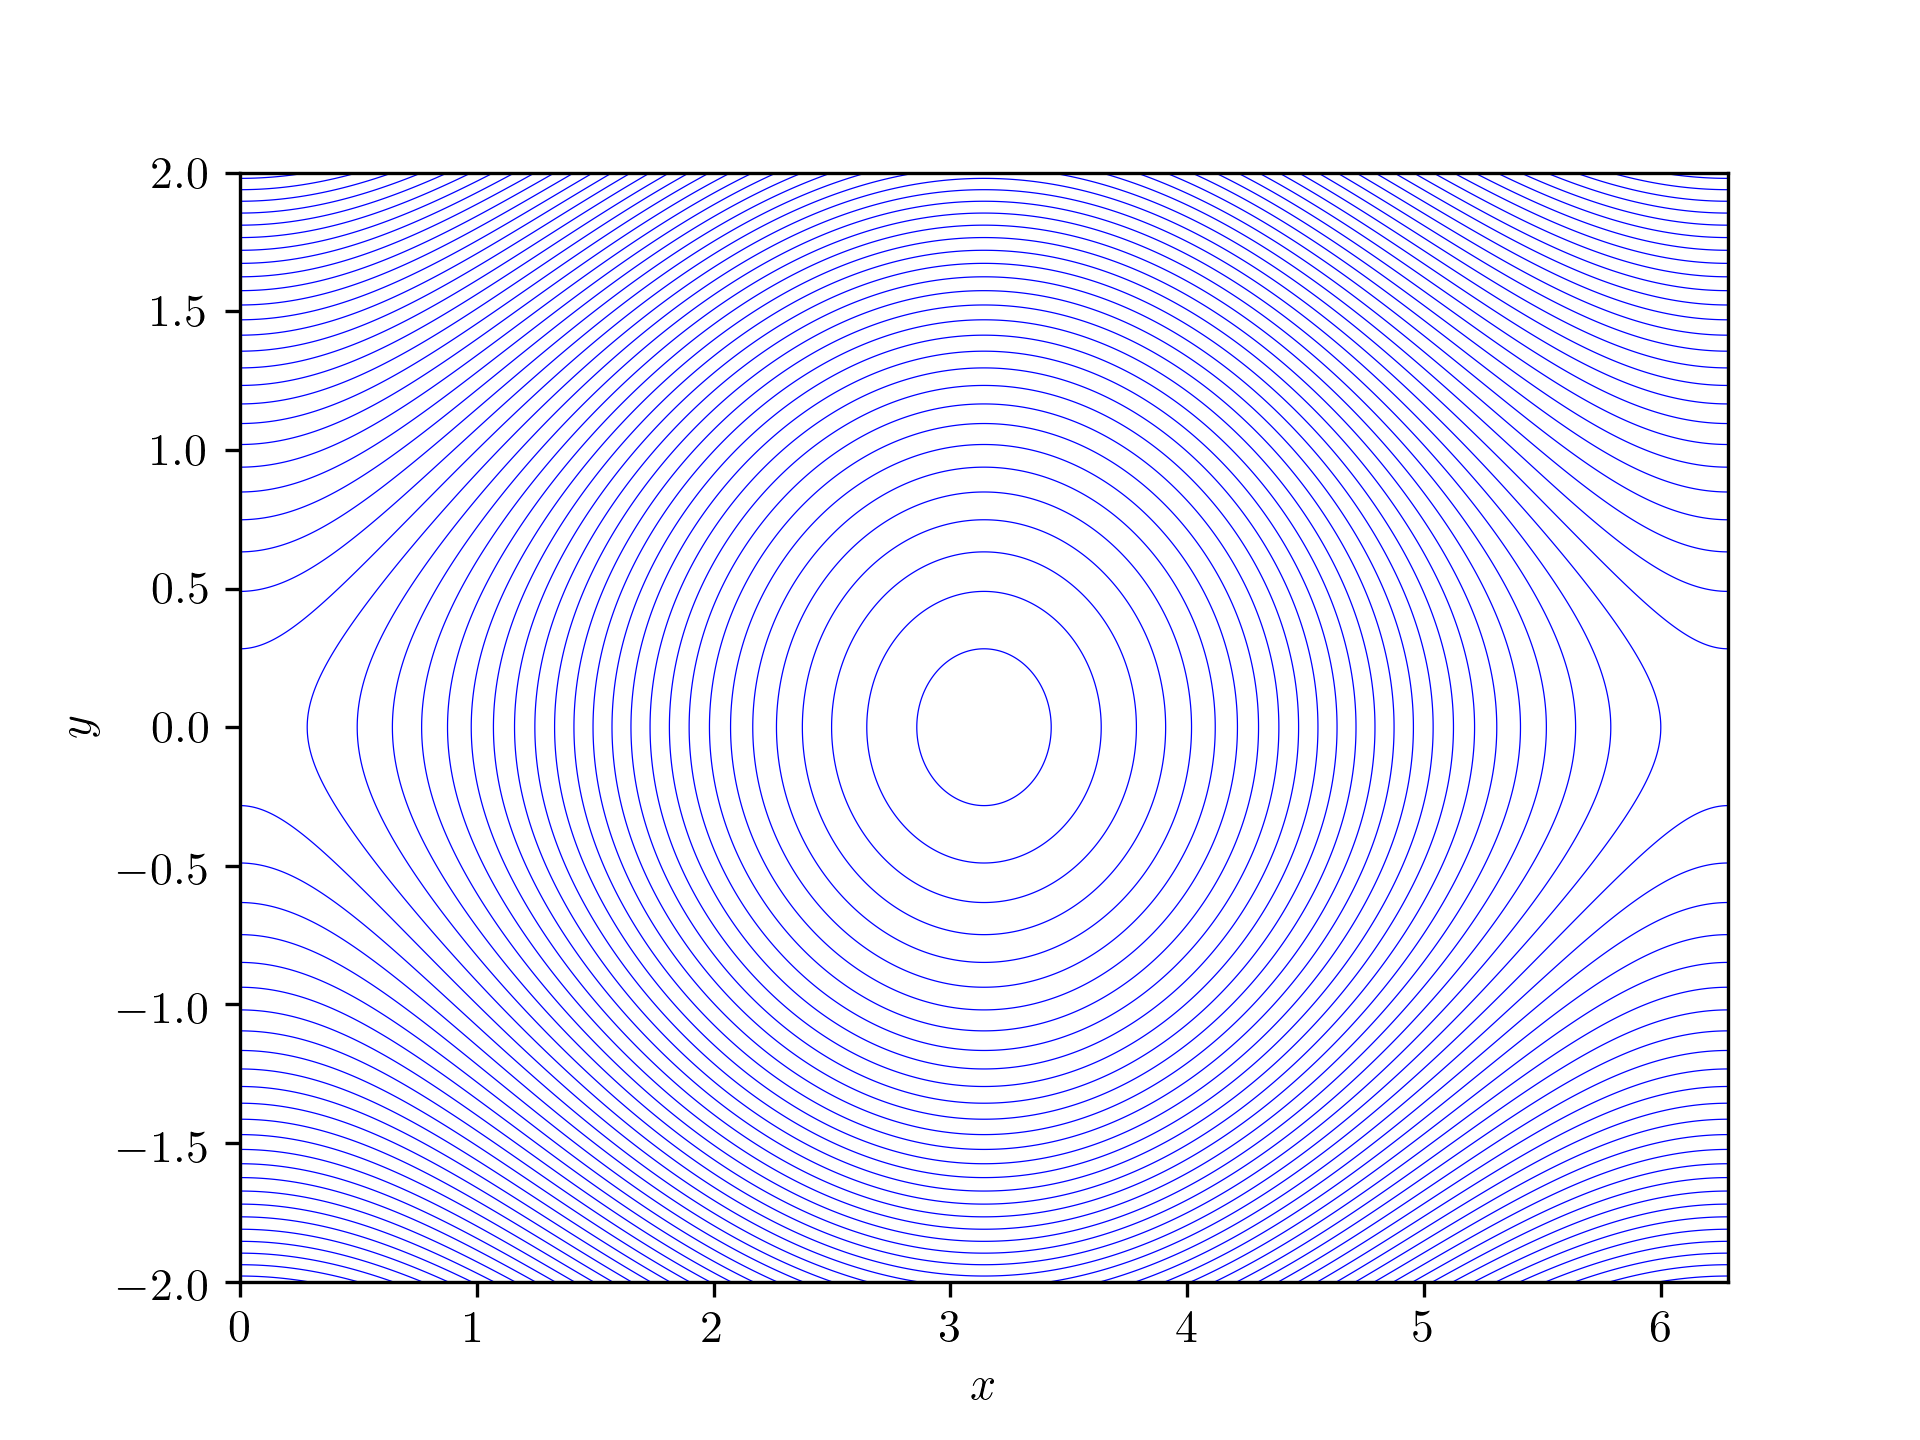
\includegraphics{img/standard-map/fase-pendolo}
		\caption{Ritratto di fase del pendolo semplice}
		\label{fig:pendolo-fase}
	\end{figure}
	
	\begin{figure}
		\centering
		\subfloat{%
			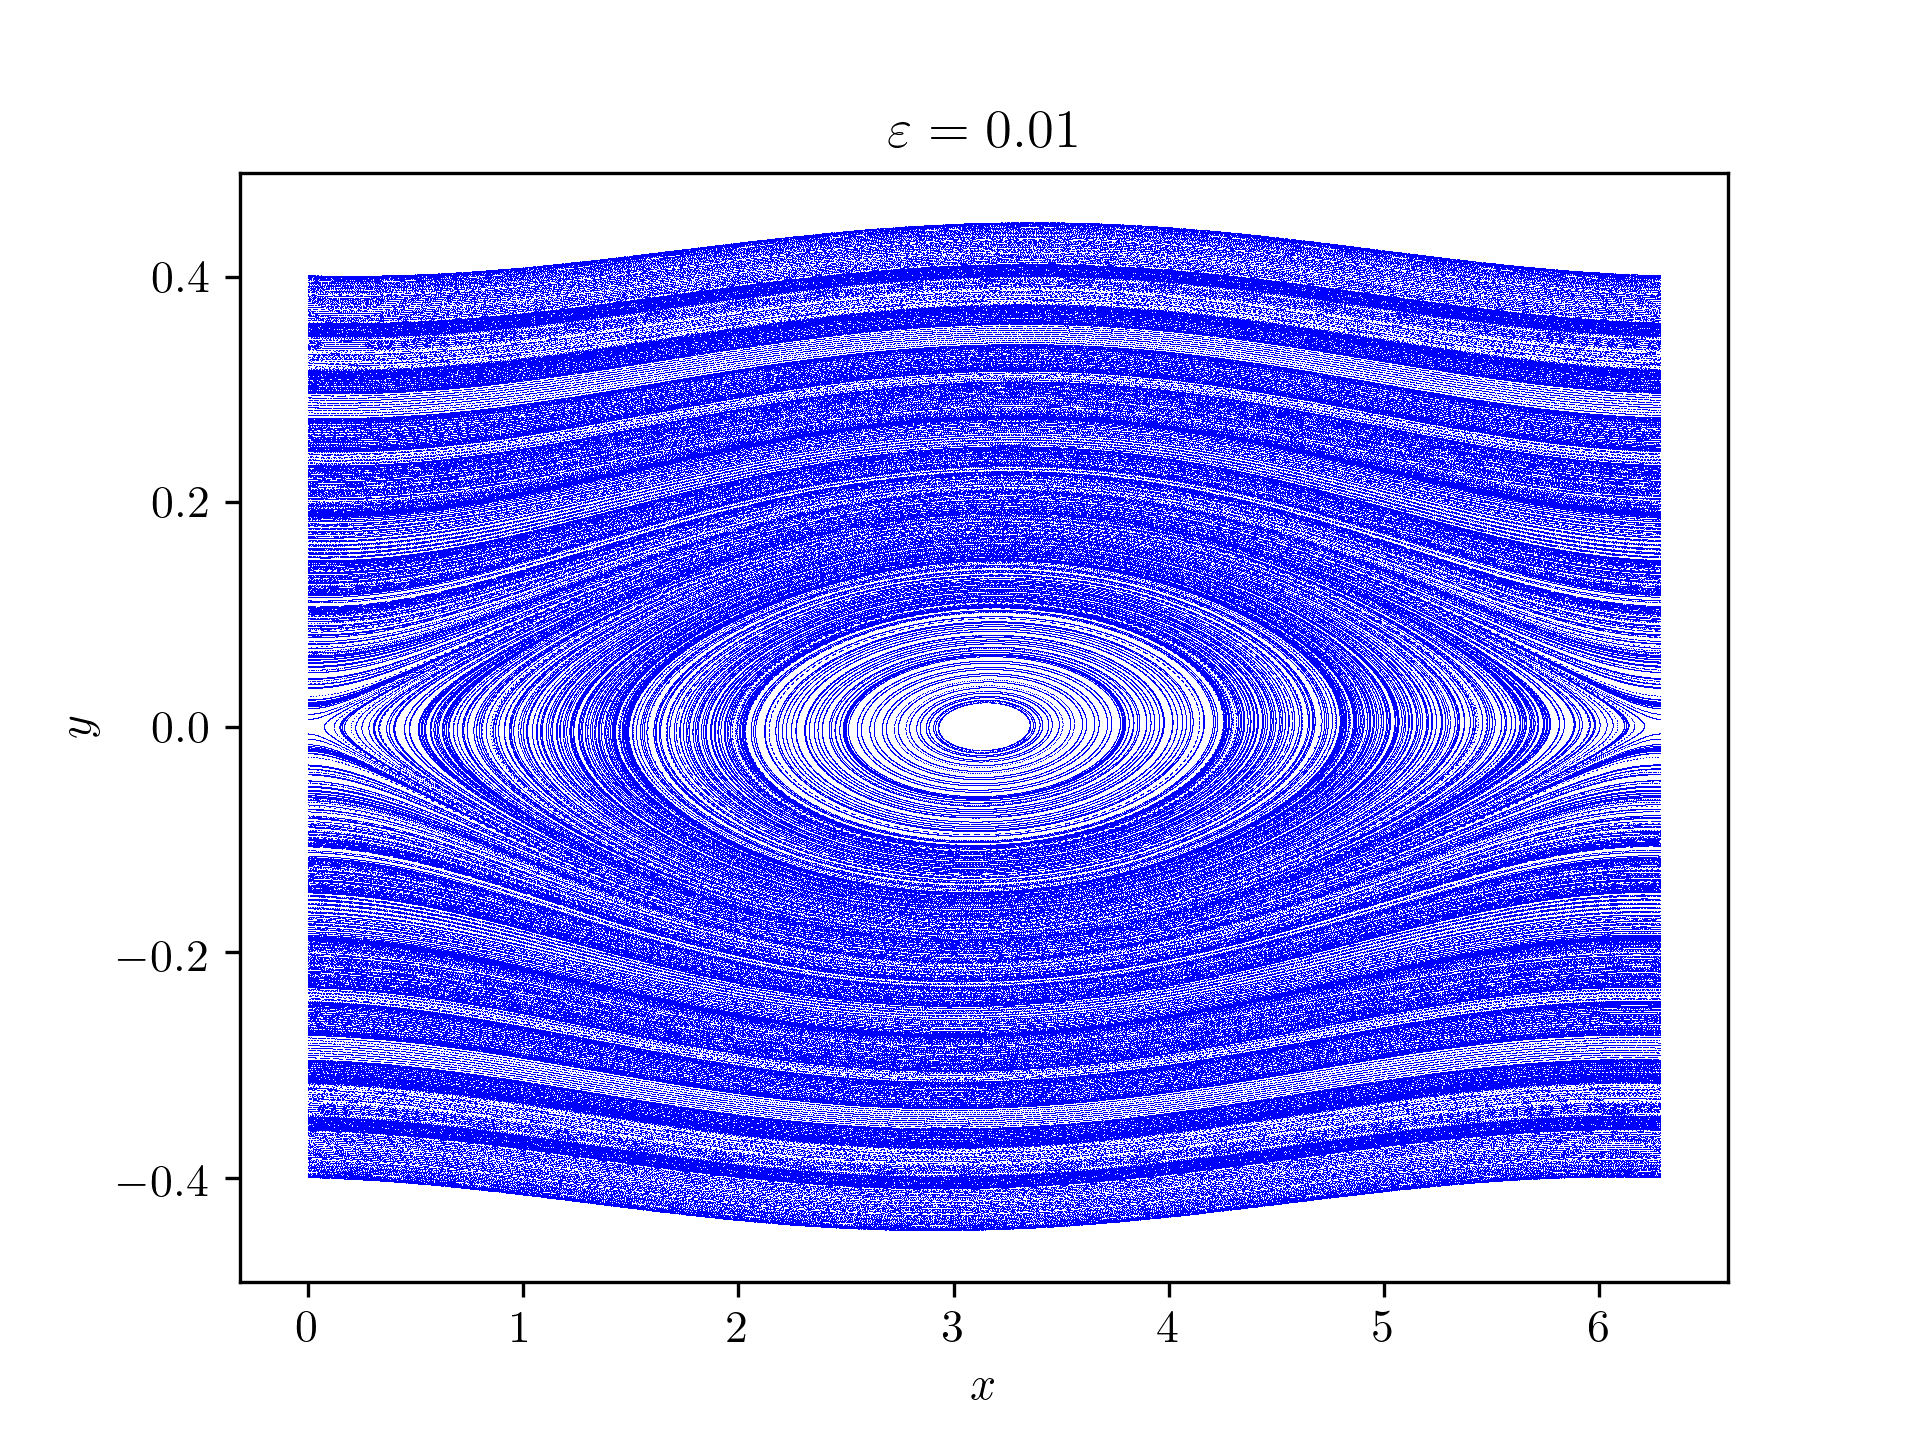
\includegraphics[width=0.5\textwidth]{img/standard-map/sm0}%
		} 
		\subfloat{%
			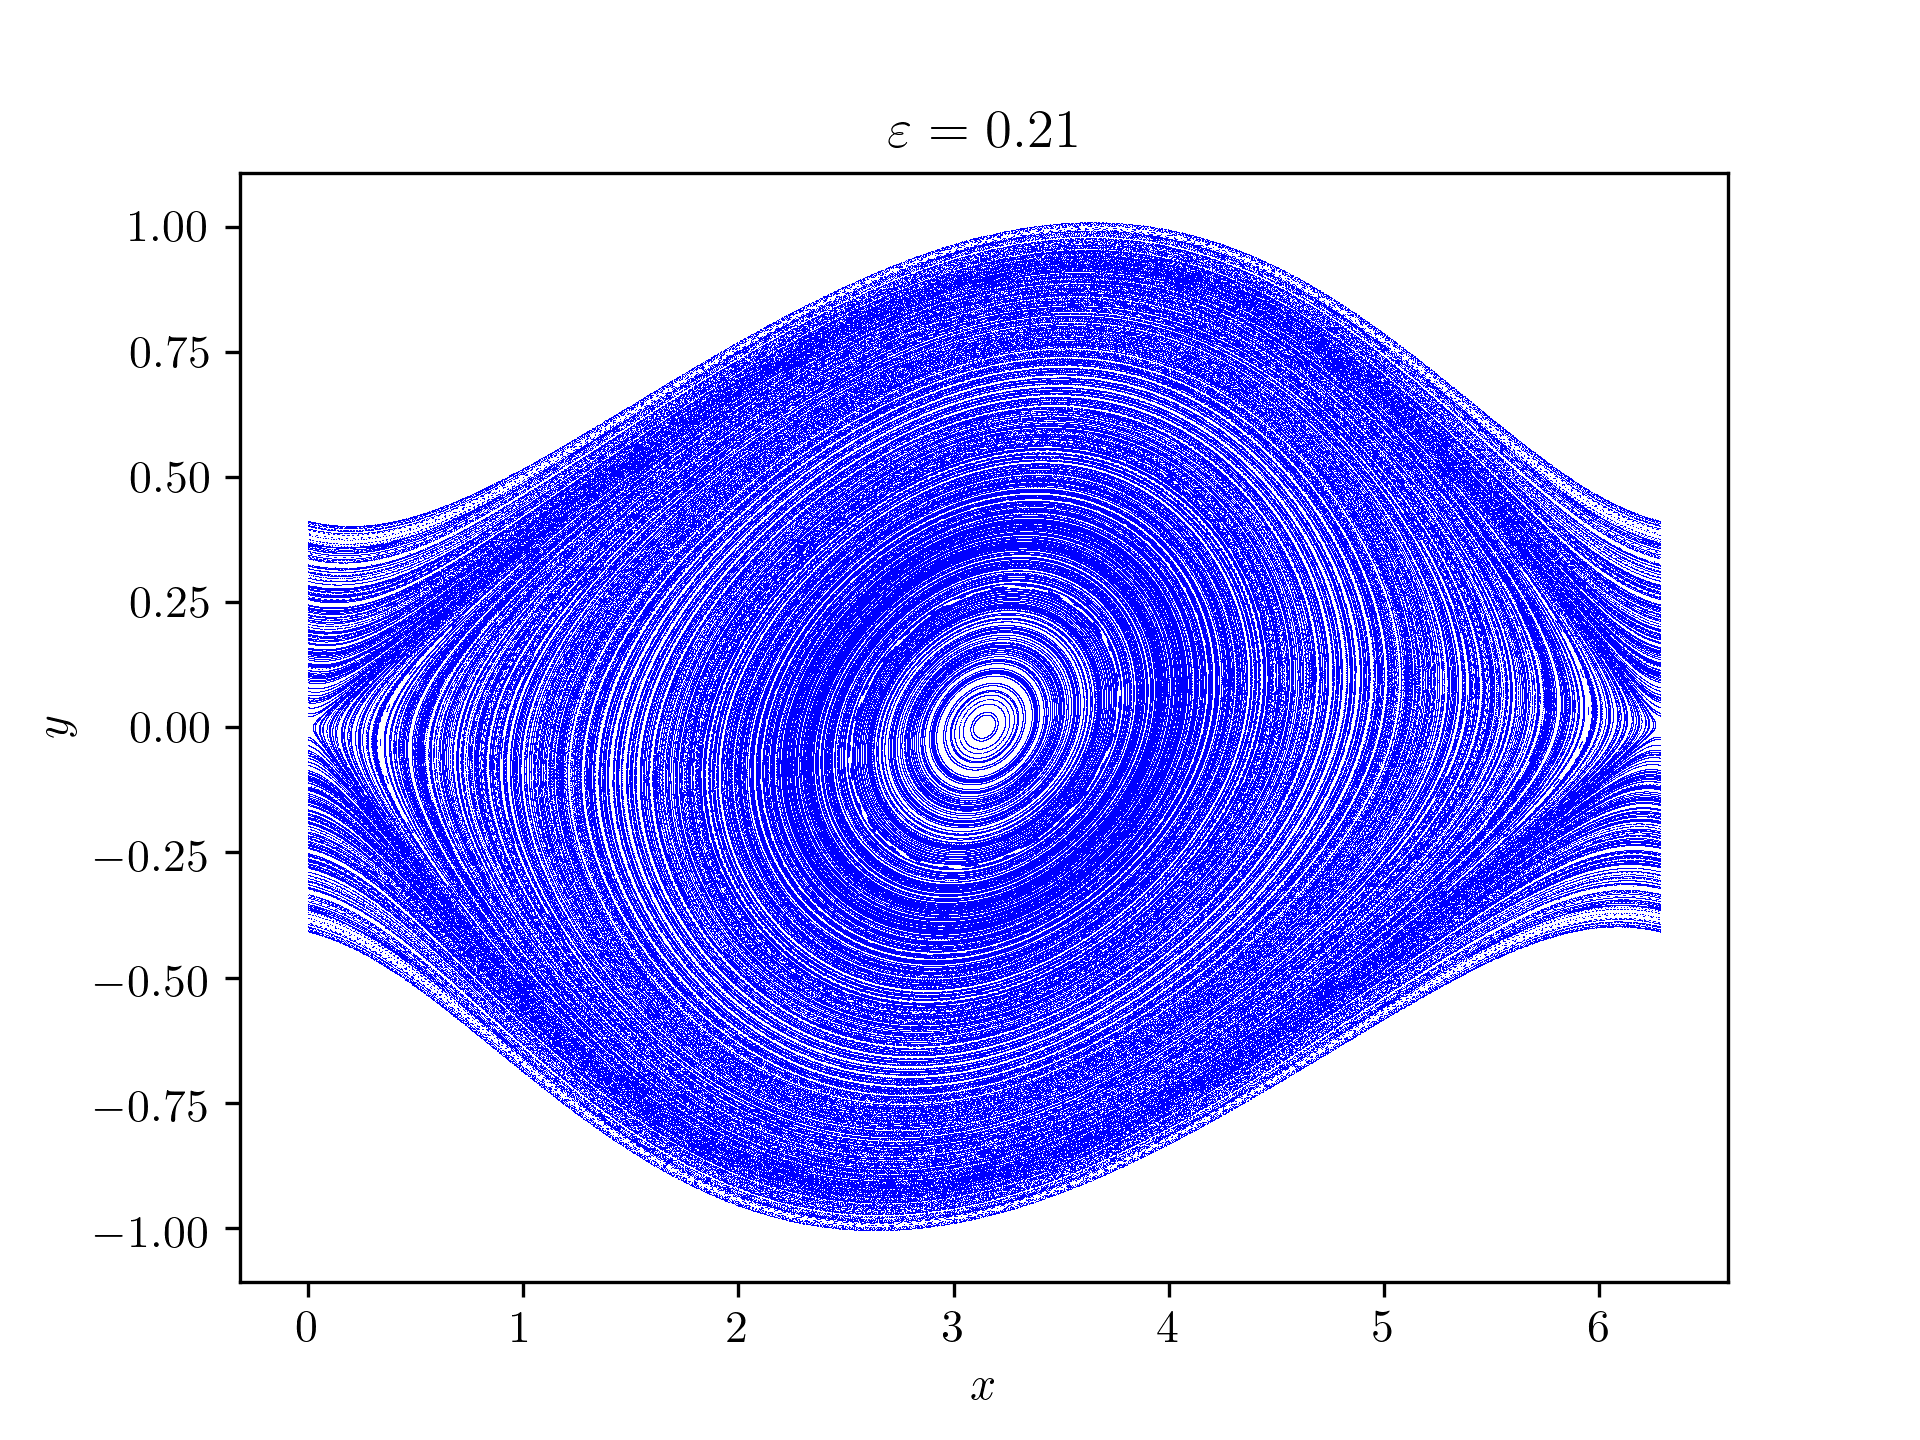
\includegraphics[width=0.5\textwidth]{img/standard-map/sm1}%
		} \hfill
		\subfloat{%
			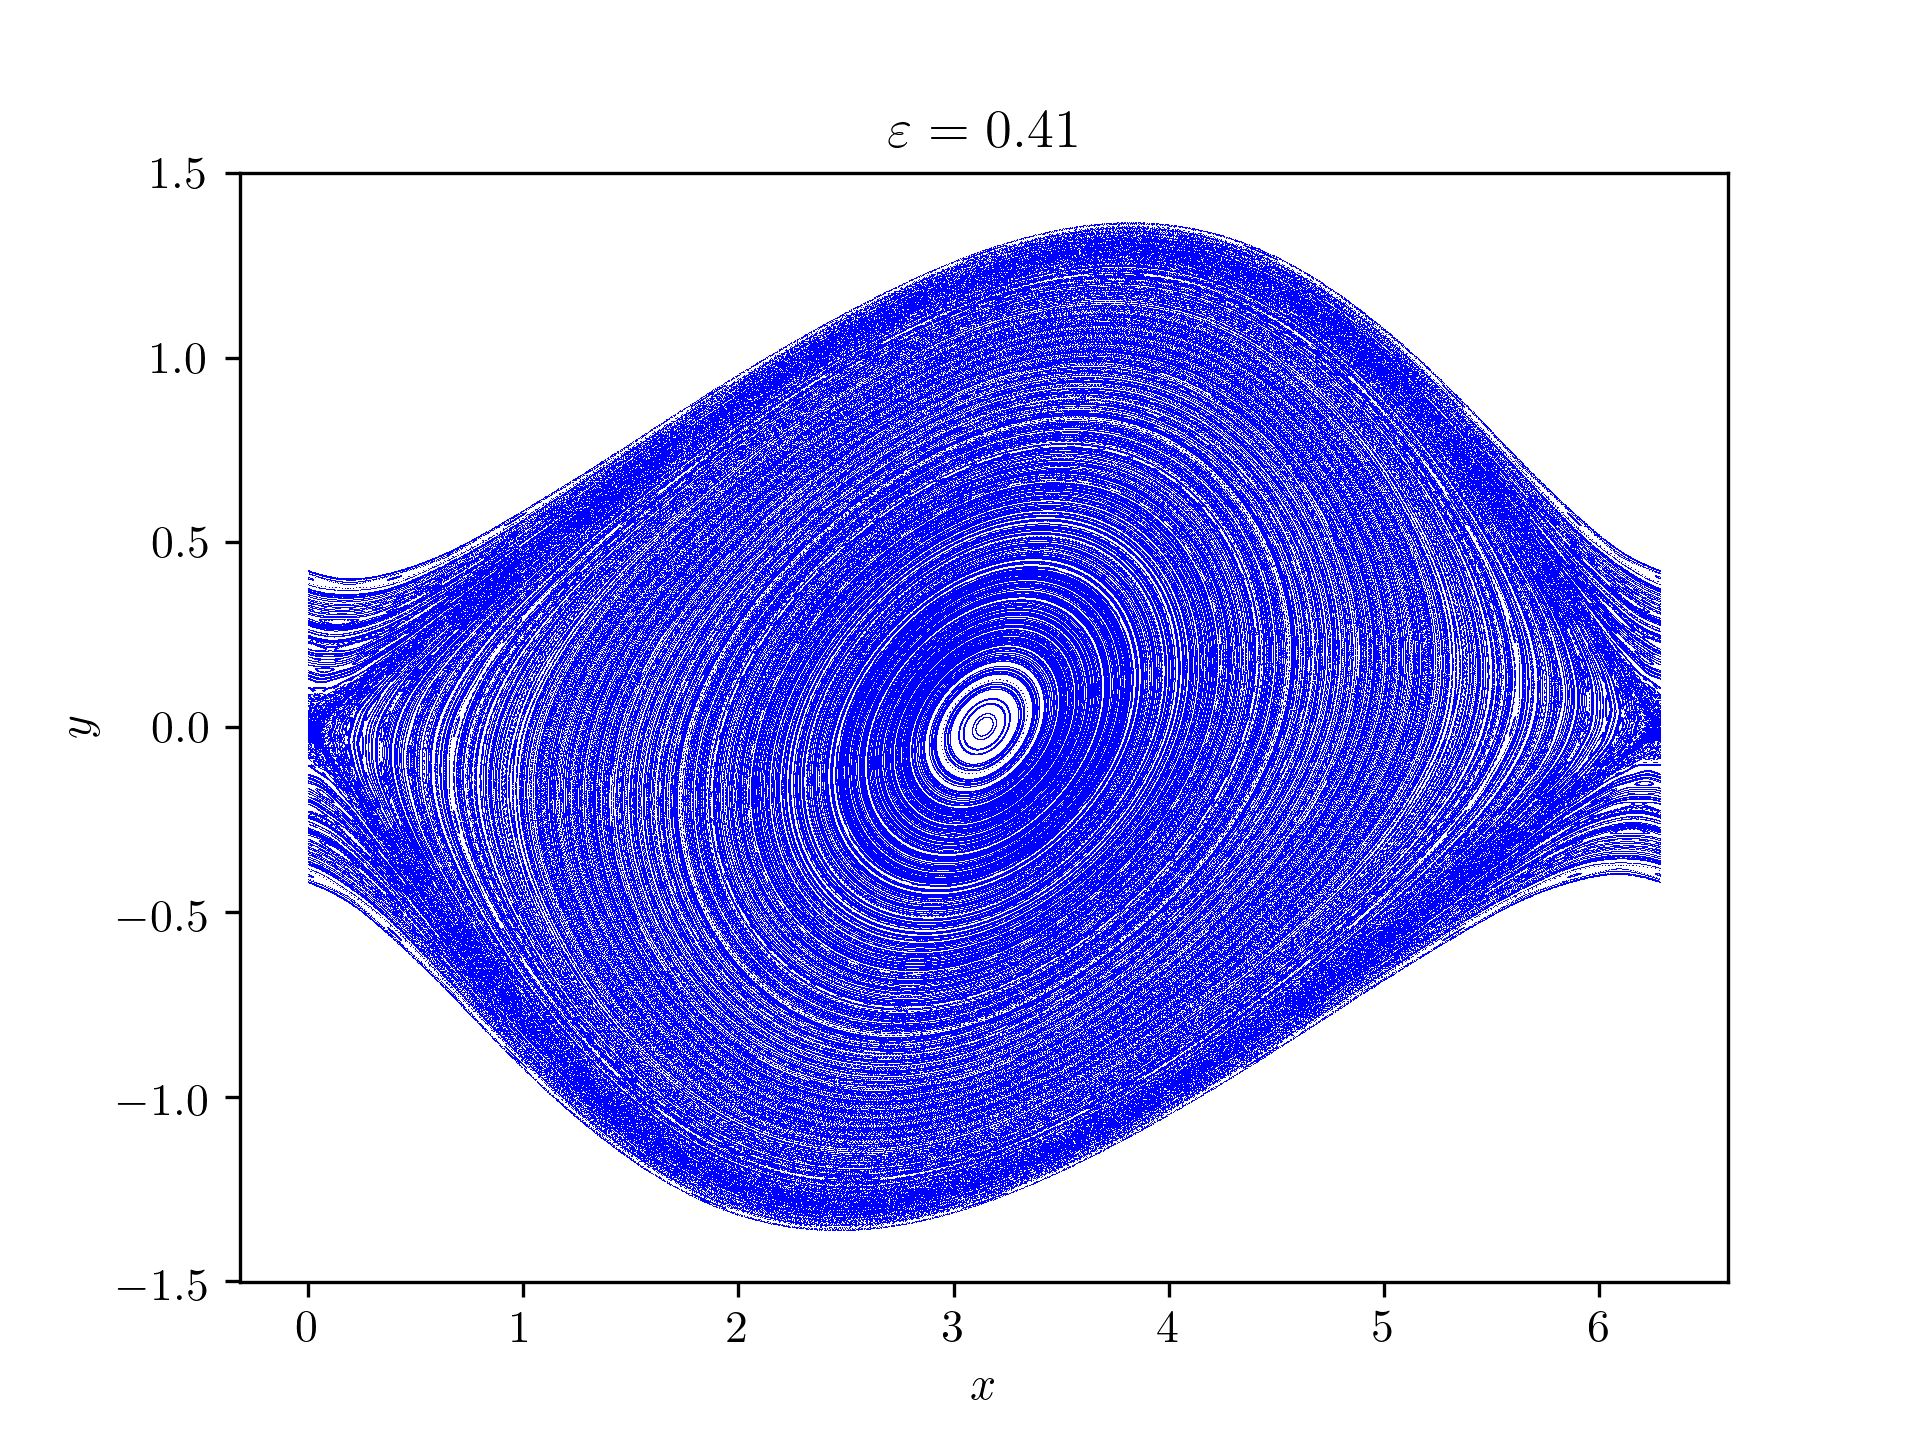
\includegraphics[width=0.5\textwidth]{img/standard-map/sm2}%
		} 
		\subfloat{%
			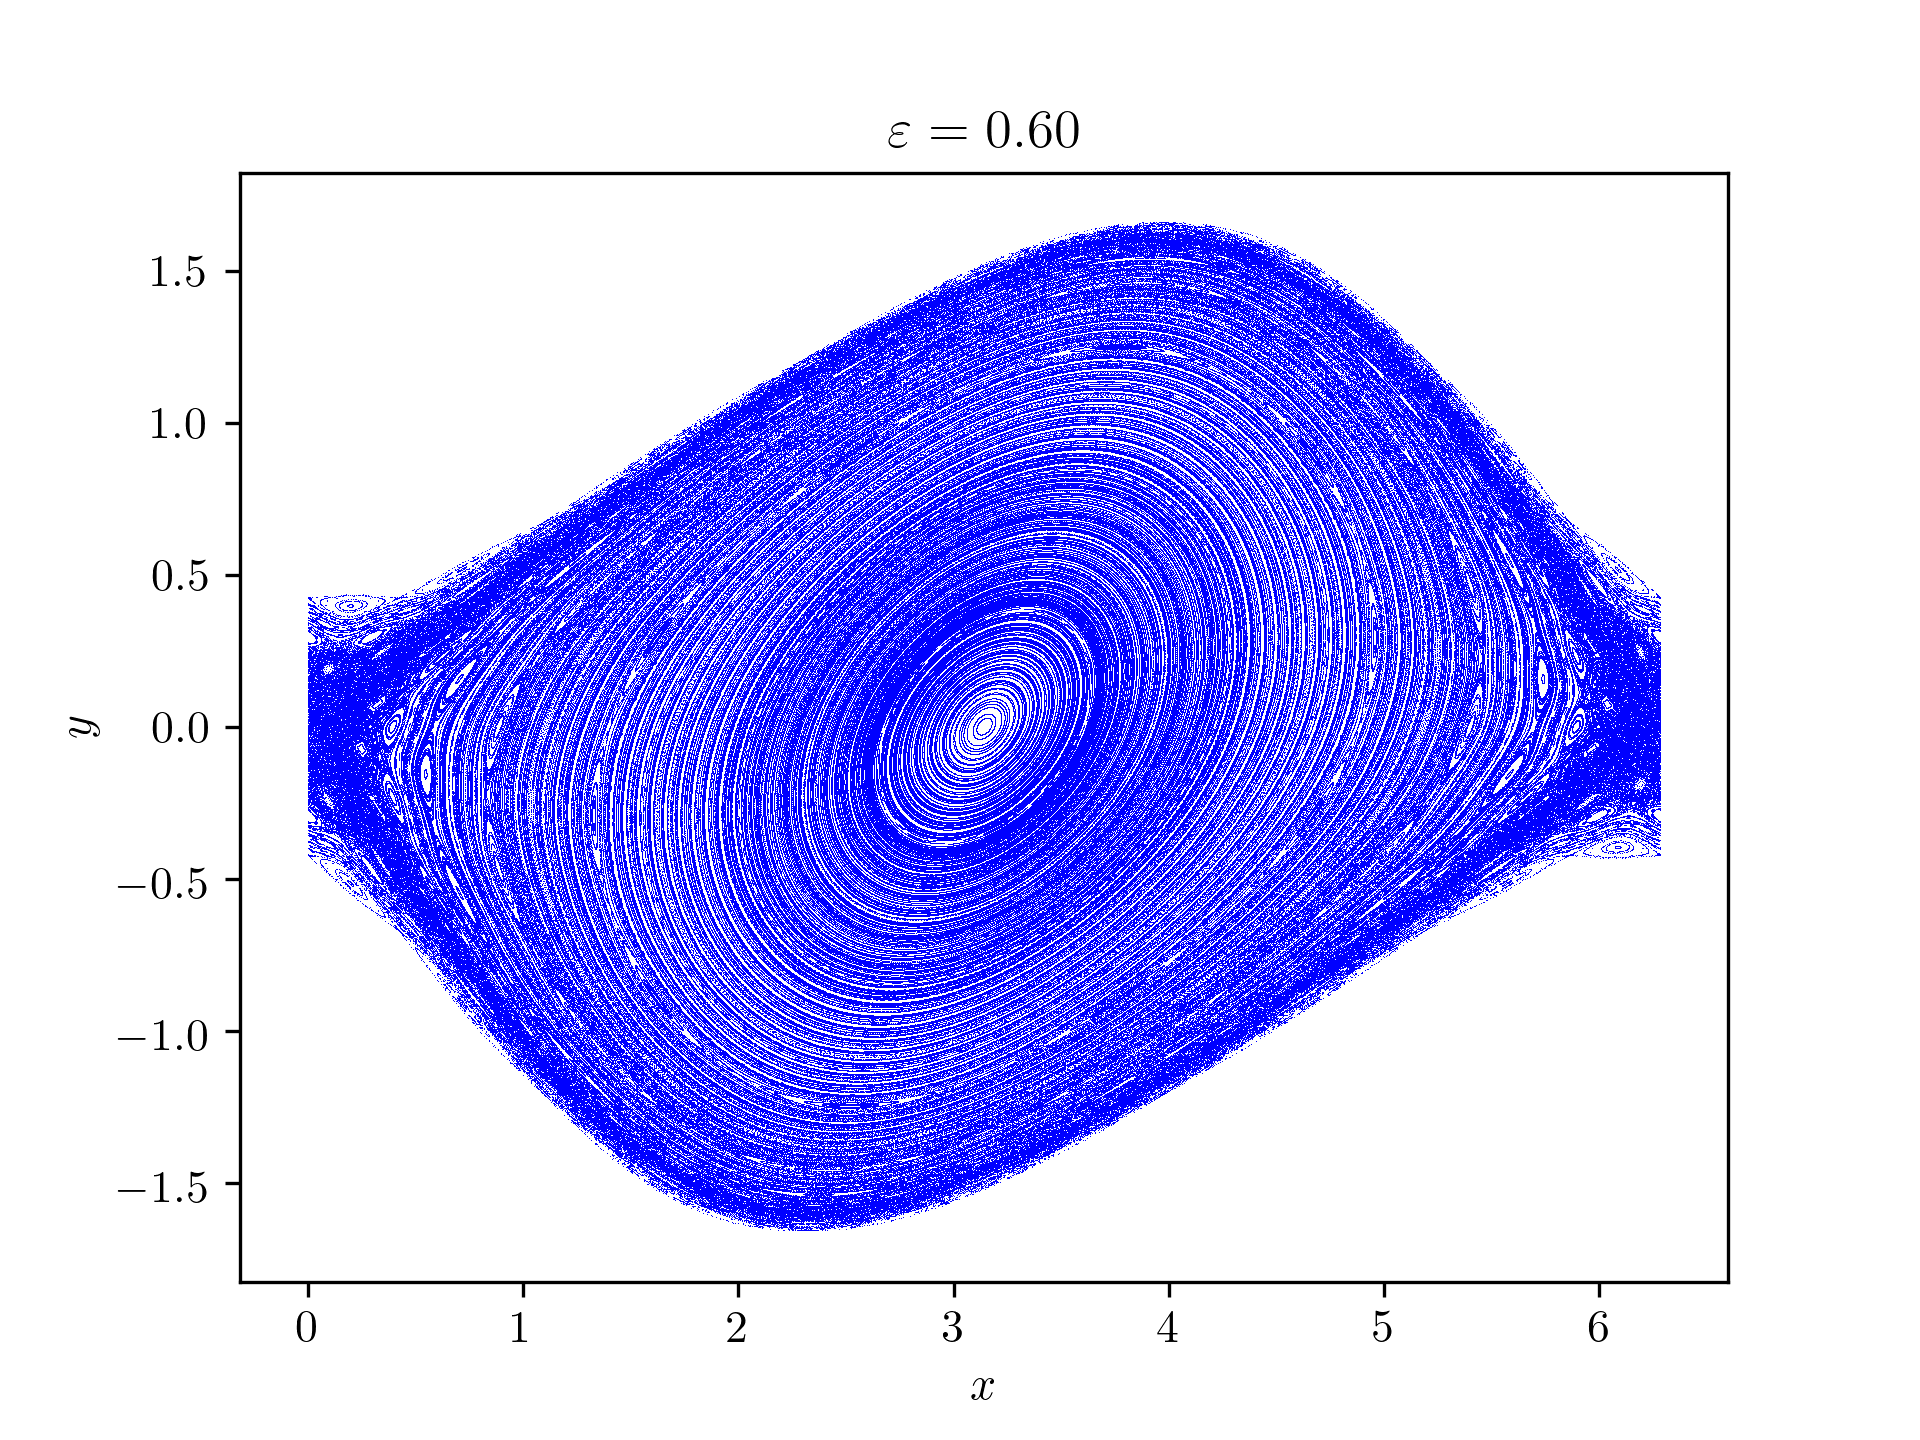
\includegraphics[width=0.5\textwidth]{img/standard-map/sm3}%
		} \hfill
		\subfloat{%
			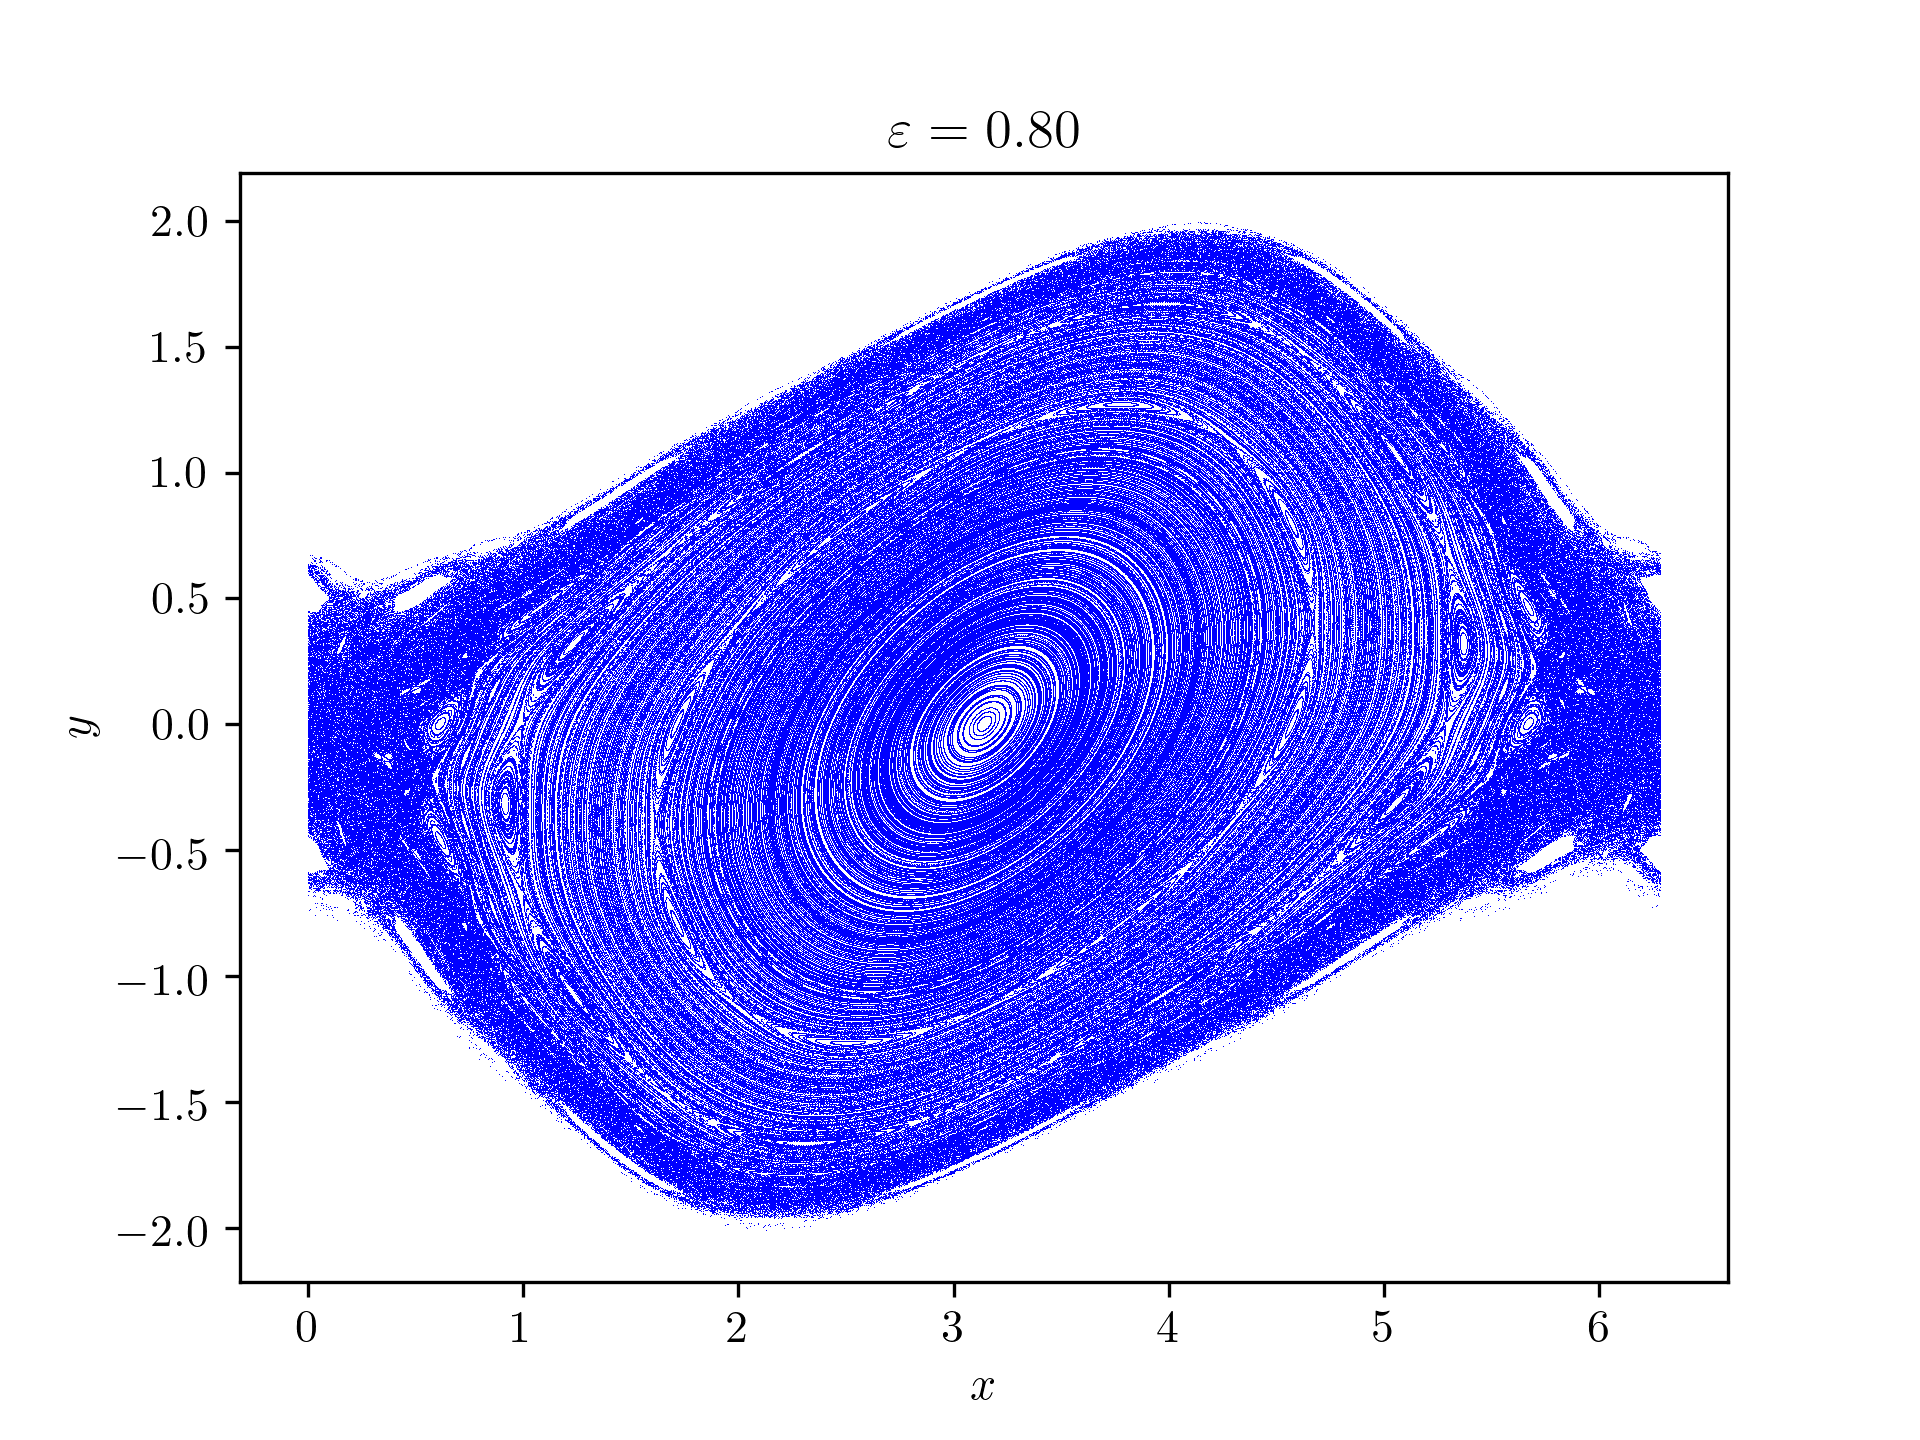
\includegraphics[width=0.5\textwidth]{img/standard-map/sm4}%
		} 
		\subfloat{%
			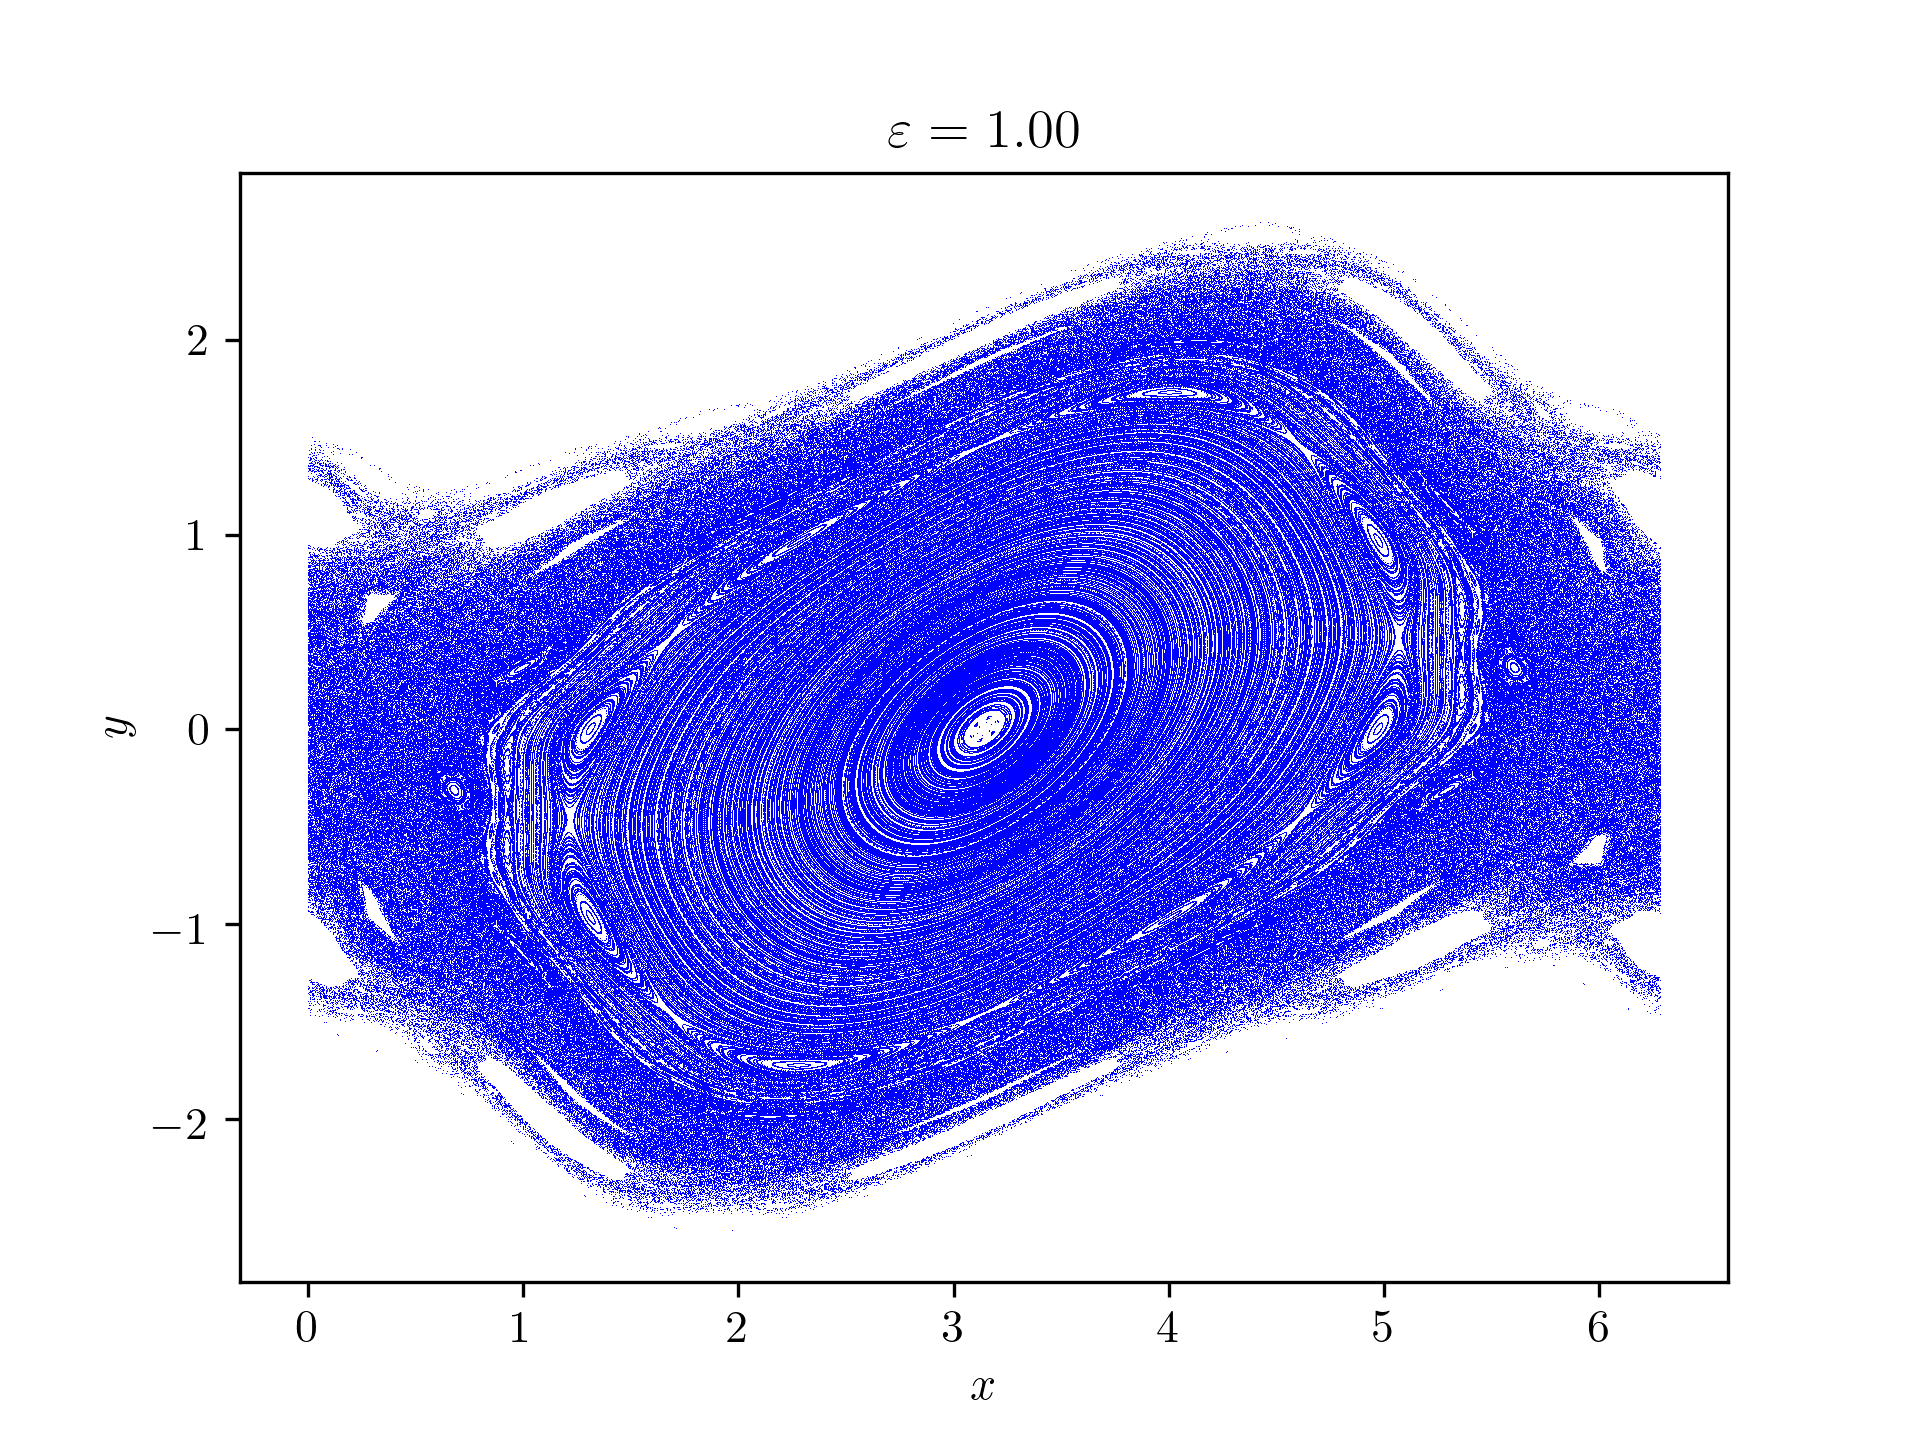
\includegraphics[width=0.5\textwidth]{img/standard-map/sm5}%
		} \hfill
		\caption{Equazione del pendolo discretizzazione per diversi valori di $ \epsilon $}
		\label{fig:pendolo-ode-num}
	\end{figure}
	\fi
	
\end{example}
